% !TEX program = xelatex
% 使用 texlive 完整编译:
% xelatex -> bibtex -> xelatex -> xelatex
% SHNU-Thesis 上海师范大学研究生毕业论文 LaTeX 模板

\documentclass[master]{shnuthesis}
% master 硕士学位论文, 默认可省略
% doctor 博士学位论文, 不能省略
% arts 文科学位论文, 默认缺省为理科
% print 用于打印, 封面等生成空白页
% 提交给图书馆的电子版不要选 print

%----- 论文标题、作者、导师、日期等相关信息 -----
\title{加性噪声驱动的时间变换随机微分方程的数值方法}
\author{左~~如~~春}   % 作者姓名
\date{二~~〇~~二~~四~~年~~九~~月 }  % 完成日期
\institute{数~~理~~学~~院}  % 学院名称
\major{计~~算~~数~~学}  % 专业名称
\research{随~~机~~微~~分~~方~~程~~数~~值~~解}  % 研究方向
\studentID{222200595}  % 学号
\shnucode{10270}  % 学校代码
\advisor{刘~~暐~~~~副~~研~~究~~员}  % 导师姓名

%----- 设置英文字体 -----
%\usepackage{newtxtext}  % New TX font for text
%\setmainfont{TeX Gyre Termes}  % Times New Roman 的开源复刻版本
%\setsansfont{TeX Gyre Heros}   % Helvetica 的开源复刻版本
%\setmonofont{TeX Gyre Cursor}  % Courier New 的开源复刻版本
\setmainfont{Times New Roman}
\setsansfont{Arial}
%\setmonofont{Courier New}

%----- 设置数学字体 -----
%\usepackage{newtxmath}
%\usepackage{mathptmx}

%----- 添加其他宏包 -----
%\usepackage[notcite,notref]{showkeys}
\usepackage{listings}
\usepackage{subfig}
\usepackage{cleveref}

%----- 取消链接颜色和方框 -----
%\hypersetup{hidelinks}

%----- 参考文献格式 -----
%\bibliographystyle{plain} % abbrv, unsrt, siam
\bibliographystyle{shnuthesis-numeric}
%\bibliographystyle{shnuthesis-author-year}

%----- 参考文献引用格式 -----
\citestyle{numbers}
%\citestyle{super}
%\citestyle{authoryear}

%----- 调整列表项的间距 -----
%\setlength{\itemsep}{3pt}

%----- 调整页面避免出现过大空白 -----
%\raggedbottom

%----- 定义符号描述命令  -----
\newcommand{\nameditem}[3][]{
\noindent\hspace{2em}\makebox[0.2\textwidth][l]{#2}{{#3}
\hfill\makebox[0.2\textwidth][l]{#1}\hspace*{2em}}\par}

%----- 微分算子 -----
\newcommand*{\dif}{\mathop{}\!\mathrm{d}}

%----- 自定义命令 -----
\newcommand{\CC}{\ensuremath{\mathbb{C}}}
\newcommand{\RR}{\ensuremath{\mathbb{R}}}
\newcommand{\A}{\mathcal{A}}
\newcommand{\bA}{\boldsymbol{A}}
\newcommand{\ii}{\mathrm{i}\mkern1mu}
\newcommand{\abs}[1]{\lvert#1\rvert}
\newcommand{\norm}[1]{\left\lVert#1\right\rVert}
\newcommand{\dx}[1][x]{\mathop{}\!\mathrm{d}#1}
\newcommand{\red}[1]{\textcolor{red}{#1}}

% 自定义标签名称
\crefname{theorem}{定理}{定理}
\Crefname{theorem}{定理}{定理}
\crefname{lemma}{引理}{引理}
\Crefname{lemma}{引理}{引理}
\crefname{corollary}{推论}{推论}
\Crefname{corollary}{推论}{推论}
\crefname{proposition}{命题}{命题}
\Crefname{proposition}{命题}{命题}
\crefname{assumption}{假设}{假设}
\Crefname{assumption}{假设}{假设}
\crefname{definition}{定义}{定义}
\Crefname{definition}{定义}{定义}
\crefname{Example}{例子}{例子}
\Crefname{Example}{例子}{例子}
\crefname{remark}{注释}{注释}
\Crefname{remark}{注释}{注释}
\Crefname{figure}{图}{图}
\crefname{figure}{图}{图}
% 自定义 cref 对 equation 环境的标签格式,仅显示编号
\crefformat{equation}{(#2#1#3)}
\crefrangeformat{equation}{(#3#1#4)--(#5#2#6)}


\begin{document}

% 生成封面页
\maketitle
% 也可以插入封面 cover.pdf 替换原始封面
%\insertcover{cover.pdf}

% 生成独创性与授权声明页, 此页可以放在最后
\makestatement
% 将签字扫描的声明页 statement.pdf 替换原始页面
%\makestatement[file=statement.pdf]

%=============== 摘要 =================%

% 关闭章节编号, 页码使用罗马数字
\frontmatter

% 中文摘要内容和关键字

% 中文摘要和关键字

\begin{cnabstract}

%研究Back-Euler-Maruyama (BEM)数值逼近一类经过Lamperti变换后,漂移系数线性增长、扩散系数是常数的时变随机微分方程.证明了BEM的强收敛性与逆从属的稳定指数之间的关系,并讨论收敛速度.并通过数值模拟验证了理论结果.

本研究提出了一种新的数值方法,专门针对一类具有高度非线性的时间变换随机微分方程(SDE)。这些SDE的漂移项和扩散项系数,满足超线性增长条件。通过应用Lamperti变换,我们将这些方程中的乘性噪声转换为加性噪声,从而简化了数值解的计算并提高了收敛阶。本研究不仅探讨了变换后的SDEs的强收敛性,还详细分析了收敛阶。此外,我们还通过数值模拟验证了理论结果的有效性,展示了该方法在提高收敛阶方面的显著优势,为时间变换SDEs的数值分析提供了新的视角和工具。



\cnkeywords{时间变换;等距离散;收敛阶;逆从属;EM型数值方法;Lamperti变换;强收敛}

\end{cnabstract}



% 英文摘要内容和关键字

%%%%%%%%%%%%% 英文摘要内容和关键字 %%%%%%%%%%%%

\begin{enabstract}
Time-changed stochastic differential equations (SDEs) are widely used in financial market modeling as an important tool to describe sub-diffusion phenomena. Therefore, research on numerical methods of time-changed stochastic differential equations has attracted much attention. Traditional solution methods mainly include classic explicit methods such as Euler-Maruyama method and Milstein method. Time-changed stochastic differential equations which coefficients satisfy global Lipschitz are usually numerically approximated by classical explicit methods that are simple, easy to implement, and highly computationally efficient. However stochastic differential equations with superlinear growth terms, the classic explicit methods tend to diverge.

This paper proposes a truncated Milstein method for a class of highly nonlinear non-autonomous stochastic differential equations with time-changed processes, using the idea of truncation to suppress superlinear growth terms. This method retains the advantages of the explicit method. The article proves strong convergence in a finite time interval properties, and obtained the convergence order. 

In a class of time-changed stochastic differential equations studied in this article, the spatial variables in the drift and diffusion coefficients satisfy the superlinear growth condition, and the temporal variables satisfies the H{\"o}lder continuity condition. In addition, the duality principle does not apply to these types of time-changed stochastic differential equations, so the connection between the classical stochastic differential equations and the time-changed stochastic differential equations cannot be established, so we can only directly construct a numerical method for the time-changed stochastic differential equations. In this paper, by constructing the truncated Milstein method,
and it is proven that the convergence order of this numerical method is ${\min\{\gamma_f,\gamma_g,(1-2\varepsilon)\}}$, where $\gamma_f$ and $\gamma_g$ represents the H{\"o}lder exponents of the temporal variables and $\varepsilon$ is an arbitrarily small number. This conclusion implies that the convergence order of the truncated Milstein method is related to the smoothness of the temporal variables. When the smoothness is poor, the convergence order of the numerical method is determined by the H{\"o}lder exponents of the temporal variables. When the smoothness is good, the convergence order of this method approaches 1. At the end of the paper, the theoretical results of numerical examples of one-dimensional and two-dimensional time-changed stochastic differential equations through Matlab were verified.

\enkeywords{time-changed stochastic differential equations; highly non-linear;  non-autonomous; Milstein-type method; strong convergence}

\end{enabstract}



%=============== 目录 =================%

% 生成目录
\maketoc

% 生成插图清单, 如不需要可以注释
%\makelof

% 生成表格清单, 如不需要可以注释
%\makelot

%=====================================%

% 主要符号表, 如不需要可以注释
%
%%%%%%%%%%%%%%%%% 主要符号表 %%%%%%%%%%%%%%%%%

% 没有主要符号表的可以直接注释此环境或删除此环境

%\begin{denotation}

%如不加特殊说明, 本论文采用如下符号和记号

%自定义命令 \verb|\nameditem[]{}{}|, 比如 \verb|\nameditem[单位]{符号}{描述}|

%\nameditem[\textbf{单位}]{\textbf{符号}}{\textbf{描述}}
%\nameditem[$\mathrm{m^{2} \cdot s^{-2}}$]{$E$}{系统的能量}
%\nameditem[$\mathrm{m\cdot s^{-1}}$]{$c$}{真空中光速}
%\nameditem[$\mathrm{m^{3}\cdot kg^{-1} \cdot s^{-2}}$]{$g$}{引力常数~(Gravitational constant)}

%\nameditem{\textbf{符号}}{\textbf{描述}}
%\nameditem{$\mathbb{R}$}{实数集}
%\nameditem{$\mathbb{R}^{n}$}{$n$ 维实向量空间}
%\nameditem{$\mathbb{C}_{+}$}{正整数集}
%\nameditem{$\mathbb{Z}$}{整数集}
%\nameditem{$\|\cdot\|_2$}{$2$-范数}
%\nameditem{$\|\cdot\|_{\infty}$}{$\infty$-范数}
%\nameditem{$A^{-1}$}{矩阵 $A$ 的逆}
%\nameditem{$A^{*}$}{矩阵 $A$ 的共轭转置}

%\vspace{2em}
%\nameditem{\textbf{缩写}}{\textbf{全称}}
%\nameditem{ODE}{Ordinary differential equation}
%\nameditem{PDE}{Partial differential equation}
%\nameditem{CFD}{Computational fluid dynamics}
%\nameditem{FDM}{Finite difference method}
%\nameditem{FEM}{Finite element method}

%\vspace{1em}
%使用 table 和 tabular 环境排版符号和描述.
%\begin{table}[htp!]
%\centering
%\renewcommand\arraystretch{1.5} %定义表格高度
%\setlength\tabcolsep{10pt} %调节列间距
%\begin{tabular}{ll}
%  \textbf{符号} & \textbf{描述} \\
%  $\mathbb{R}$  & 实数集   \\
%  $\mathbb{R}^{n}$  & $n$ 维实向量空间   \\
%  $\mathbb{C}_{+}$  & 正整数集  \\
%  $\mathbb{Z}$  & 整数集  \\
%  $\|\cdot\|_2$  & $2$-范数   \\
%  $\|\cdot\|_{\infty}$  & $\infty$-范数   \\
%  $A^{-1}$  & 矩阵 $A$ 的逆  \\
%  $A^{*}$   & 矩阵 $A$ 的共轭转置
%\end{tabular}
%\end{table}

%\end{denotation}



%============== 正文部分 ==============%

% 开启章节编号, 页码使用阿拉伯数字
\mainmatter

% 第1章 引言

% 引言

\chapter{引言}\label{chap:Intro}

\section{研究背景}\label{sec:background}




受到\cite{Alfonsi2013602}的启发,本文的目的是推导出一个有效的数值逼近一类一维随机微分方程.这类随机微分方程可以通过Lamperti变换,将漂移项变换成满足单调条件的,见\cite{iacus2008simulation},通过BEM对变换后的时变SDE进行逼近,再将其变换成原始时变SDE的逼近格式.

对于Lamperti变换的随机微分方程, 截止目前已经有了很多结果.\cite{neuenkirch2014first}研究了一大类Lamperti变换后随机微分方程的漂移项是局部Lipschitz的,并得到1阶的强收敛阶. \cite{yang2021first}研究了Lamperti变换作用在SIS模型中,并且得到1阶强收敛阶

对于时间变换的随机微分方程,有关收敛阶的研究,截止目前已经有而很多结果.\cite{wen2023strong}
研究了非自治的时间变换McKean-Vlasov随机微分方程,并给出EM方法的强收敛性和收敛阶.\cite{liu2020truncated}.研究截断EM方法来逼近一类具有Hölder连续性和超线性增长的非自治随机微分方程,并证明了强收敛性和收敛阶.\cite{jin2021strong}
研究一类具有时间变换Lipschitz界限下,包含随机和非随机积分项的时间变换随机微分方程,并讨论EM方法和Ito-Taylor方法的强收敛性和收敛阶.\cite{li2023convergence}
研究一类具有超线性增长的,包含随机和非随机积分项的时间变换随机微分方程,并讨论截断EM方法的强收敛性和收敛阶.在\cite{jum2014strong}中证明了对于漂移项和扩散项都满足全局Lipschitz时,可以采用对偶原则,将时间变换随机微分方程转换成一般随机微分方程,通过对一般随机微分方程使用EM数值格式进行逼近,进而得到时间变换随机微分方程的强收敛阶.在\cite{deng2020semi}中将这一思想运用在漂移项满足非全局Lipschitz条件时,使用半隐式EM得到强收敛阶,并研究了其稳定性.这解决了一大类可以对偶化的时间变换微分方程的数值格式收敛性问题.在\cite{jin2019strong},对于不能使用对偶原则的时间变换随机微分方程,采用一种非等距的离散格式,并得到强收敛阶.对于时间变换的随机微分方程,现在已经有了很多的数值格式,但是到目前为止这些数值格式,大多采用的是非等距离散,对于$E(t)$的离散,通过对$t$非等距离散,使之变成实际上是对$E(t)$的等距离散.而在这篇文章中,我们将对$t$采用等距离散来研究随机微分方程:
\begin{equation}\label{basic SDE}
	dX(s)=f(X(s))dE(s)+\sigma dB(E(s))
\end{equation}
这样离散,会引入一个必须面临的困难,在取期望的时候,不能再像之前的离散那样,将微分项的$dt$拿出来,这就引入了不得不解决的麻烦,对于$dE(t)$的分析.
\cite{daley2003introduction}和\cite{magdziarz2009stochastic}中对于Cox这个更新过程的描述,对研究$E(t)$的期望起到了关键性作用.


\section{主要结论}\label{sec:mainResults}

主要结论


\section{结构安排}

本文接下来的写作安排如下:




% 第2章 LaTeX 常用环境

%%%%%%%%%%%%%%% LaTeX 常用环境 %%%%%%%%%%%%%%%

\chapter{准备工作}\label{chap:LaTeXEnv}
在这一章节中, 主要分为四个部分进行阐述:

第一部分将对本文使用的符号及其含义进行解释说明.

第二部分给出证明截断Milstein方法的收敛性并获得收敛阶所需的假设条件.

第三部分具体阐述截断函数的定义, 同时详细介绍非自治时间变换随机微分方程截断Milstein方法的构造过程.

第四部分列出一系列关键引理, 这些引理在证明截断Milstein方法的收敛阶主要结论时起到重要作用.

\section{符号说明}
在本文中, 定义 $(\Omega_W, \F^W,\PP_W)$为一个完备的概率空间, 其中$\{\F^W_t\}_{t \geq 0}$是右连续且递增的, $\F^W_0$包含所有 $\PP_W$空集, $W(t)$为该概率空间中定义的并适应$\F^W_t$的一维维纳过程, $\EE_W$表示关于$\PP_W$的期望. 定义另一个完备的概率空间$(\Omega_D, \F^D,\PP_D)$, 其中$D(t)$表示从$D(0) =0$开始在$(\Omega_D, \F^D,\PP_D)$上定义的一维$\{\F^D_t\}$适应L\'{e}vy过程, 其在$\left\{\F^D_t\right\}_{t \ge 0}$上严格递增, $\EE_D$表示关于$\PP_D$的期望. 更多关于$D(t)$的详细介绍和讨论可参考相关文献\cite{applebaum2009,ken1999}.

在本文中, 假设$W(t)$ 和 $D(t)$ 是独立的. 定义乘积概率空间$(\Omega , \F, \PP):= (\Omega_W \times \Omega_D, F^W\otimes \F^D, \PP_W \otimes \PP_D)$, $\EE$ 表示概率测度$\PP$下的期望. 显然$\EE(\cdot) = \EE_D\EE_W (\cdot) = \EE_W\EE_D (\cdot)$. 
对任意$x\in \RR^d$, $|x|$ 定义为欧几里得范数, $x^T$表示$x$的转置. 此外, 对任意两个实数 $a$和$b$, 我们使用符号$a\vee b=\max(a,b)$和$a\wedge b=\min(a,b)$. 对给定的集合 $G$, 其指示函数用$I_{G}$表示.

由于$D(t)$是严格递增的, 定义$D(t)$的反函数为
\begin{align*}
    E(t) := \inf\{ s\geq0\,;\,D(s) > t \}, \quad t \geq 0.
\end{align*}
由$t\mapsto E(t)$是连续且非递减的, $E(t)$被称为时间变换过程, $W(E(t))$被称为时间变换的维纳过程, 同时$W(E(t))$也被视为一种亚扩散过程. 为了避免复杂的符号, 在本篇文章中, 我们考虑一维的 $W(E(t))$. 当 $W(t)$是一个多维的维纳过程且相同的$E(t)$被用于 $W(t)$ 的每个分量中进行时间变换时, 本文的结果仍然成立. 但是, 如果在 $W(t)$ 的不同分量中使用不同的 $E(t)$ 进行时间变换时, 我们的结果可能不适用.

本文考虑的时间变换随机微分方程具有以下形式, 对任意$T>0$和$t\in [0,T]$,
\begin{align}\label{SDE}
    dY(t) = f(t,Y(t))dE(t) + g(t,Y(t))dW(E(t)),~~Y(0) = Y_0,
\end{align}
对所有$q > 0$都有$\EE |Y_0|^q < \infty$, 其中: $f: \RR_+ \times \RR^d \rightarrow \RR^d$ 且 $g: \RR_+ \times \RR^d \rightarrow \RR^{d}$. 

在对\eqref{SDE}的系数施加假设之前, 我们首先提出一些有用的符号, 即对任意$y=(y^{1},y^{2},...,y^{d})^{T}$和$t \in [0, T]$, 定义
\begin{align*}
    Lg(t,y)=\sum_{l=1}^{d}g^{l}(t,y)G^{l}(t,y),
\end{align*}
其中$g=(g^{1},g^{2},...,g^{d})^{T}$, $g^{l}:\RR_+ \times \RR^d \rightarrow \RR$且
\begin{align*}
    G^{l}(t,y)=(\dfrac{\partial g^{1}(t,y)}{\partial y^{l}},\dfrac{\partial g^{2}(t,y)}{\partial y^{l}},...,\dfrac{\partial g^{d}(t,y)}{\partial y^{l}})^{T}.
\end{align*}
\par

\section{假设条件}
对时间变换随机微分方程\eqref{SDE}的系数施加如下的假设. 首先, 我们对漂移项和扩散项系数中的空间变量提出假设.
\begin{assumption}
    \label{ass1}
    假设存在正常数 $\a$ 和 $C$, 使得
    \begin{equation*}
        |f(t,x)-f(t,y)|\vee |g(t,x)-g(t,y)|\vee |Lg(t,x)-Lg(t,y)|\leq C(1+|x|^{\a}+|y|^{\a})|x-y|,
    \end{equation*}
    对任意$t\in[0,T]$和$x,y \in \RR^d$成立.

    从假设\ref{ass1} 可以推出, 对任意$t\in [0,T]$和$x\in \RR^d$, 有
    \begin{equation}
        \label{equ2-2}
        |f(t,x)|\vee|g(t,x)|\vee|Lg(t,x)|\leq M(1+|x|^{\a+1}),
    \end{equation}
   其中$M$取决于 $C$ 和 $\sup_{0\leq t\leq T}\left(|f(t,0)|+|g(t,0)|+|Lg(t,0)|\right)$.
\end{assumption}
\par
\begin{assumption}
    \label{ass2}
    假设存在一对常数 $p>2$ 和 $K>0$, 使得
    \begin{equation*}
        (x-y)^{\mathrm{T}}(f(t,x)-f(t,y)) +(5p-1)|g(t,x)-g(t,y)|^2\leq K|x-y|^2,
    \end{equation*}
    对任意$t\in [0,T]$和$x,y \in \mathbb{R}^d$成立.
\end{assumption}
\begin{assumption}
    \label{ass3}
    假设存在一对常数$q>2$和$K_1>0$, 使得
    \begin{equation*}
        x^{\mathrm{T}}f(t,x) +(5q-1)|g(t,x)|^2\leq K_1(1+|x|^2),
    \end{equation*}
    对任意 $t\in [0,T]$和$x \in \mathbb{R}^d$成立.
\end{assumption}
假设\eqref{ass3}可以从假设\eqref{ass2}中推导得出, 但由于其中涉及到复杂的关系, 其中包括$p$、$q$、$K$和$K_1$之间的关系, 为简化符号, 我们将假设\eqref{ass3}提出作为一个新的假设.
\begin{assumption}
    \label{ass5}
    假设存在一个正常数$ M^{\prime}$, 使得
    \begin{eqnarray*}
        &&|\frac{\partial f(t,x)}{\partial x}|\vee|\frac{\partial^{2} f(t,x)}{\partial x^{2}}|\vee|\frac{\partial g(t,x)}{\partial x}|\vee|\frac{\partial^{2} g(t,x)}{\partial x^{2}}|\leq M^{\prime}(1+|x|^{\a+1}),
    \end{eqnarray*}
    对任意 $x\in \mathbb{R}^d$和$t\in [0,T]$成立.
        
接下来, 我们对漂移项和扩散项系数中时间变量进行假设.
\end{assumption}
\begin{assumption}
    \label{ass4}
    假设存在常数$\gamma_{f}\in (0,1]$, $\gamma_{g}\in (0,1]$, $H_1>0$ 和 $H_2>0$, 使得
    \begin{eqnarray*}
        &&|f(s,x)-f(t,x)|\leq H_1(1+|x|^{\a+1})(s-t)^{\gamma_{f}},\\
        &&|g(s,x)-g(t,x)|\leq H_2(1+|x|^{\a+1})(s-t)^{\gamma_{g}},
    \end{eqnarray*}
    对任意$x,y \in \mathbb{R}^d$ 和 $s,t\in [0,T]$成立.
    \par
\end{assumption}

\section{非自治时间变换随机微分方程的截断Milstein型方法}\label{sec:mathEqEnv}
现在我们介绍本文讨论的Milstein型方法的构造过程.
\par \noindent

{\bf 第一步}根据时间变换随机微分方程系数的形式, 我们选择一个严格递增的连续函数$\m:\RR_+\rightarrow \RR_+$, 当$u\rightarrow \infty$时$\m(u)\rightarrow \infty$, 且对任意$l = 1,2, ...,d$有
\begin{align*}
    \sup_{0\leq t\leq T}\sup_{|x|\leq u}(|f(t,x)|\vee|g(t,x)|\vee|G^{l}(t,x)|)\leq \m(u),\quad \forall u\geq 1.
\end{align*}
\par \noindent

{\bf 第二步}选择一个常数$\hat{\k}\geq 1\wedge \m(1)$ 和一个严格递减函数$\k:(0,1]\rightarrow [\m(1),\infty)$, 使得
\begin{align}
    \label{equ0}
    \quad h^{1/4}\k(h)\leq \hat{\k},\quad \forall h \in (0,1],\quad\text{且}\lim_{h \rightarrow 0}\k(h)=\infty.
\end{align}
\par \noindent

{\bf 第三步}定义$\m^{-1}$为$\m$的反函数, 显然$\m^{-1}$是一个从$[\m(0),\infty)$到$\RR_+$严格递增的连续函数. 对于给定的步长$h \in (0,1]$, 定义截断映射$\pi_{h}:\RR^d \rightarrow \{ x\in \RR^d:|x|\leq \m^{-1}(\k(h))\}$,
\begin{align*}
    \pi_{h}(x)=\left(|x|\wedge\m^{-1}(\k(h))\right)\frac{x}{|x|},
\end{align*}
当$x=0$时$x/|x|=0$. 然后通过以下方式定义截断函数:
\begin{align*}
    f_{h}(t,x)=f(t,\pi_{h}(x)),\quad g_{h}(t,x)=g(t,\pi_{h}(x)),\quad G^{l}_{h}(t,x)=G^{l}(t,\pi_{h}(x)).
\end{align*}
其中$x\in \RR^d$, $l = 1,2, ...,d$. 不难看出对任意 $t\in[0,T]$ 和$x \in \RR^d$有
\begin{align}
    \label{equ01}
    |f_{h}(t,x)|\vee |g_{h}(t,x)|\vee |G^{l}_{h}(t,x)|\leq \m(\m^{-1}(\k(h)))=\k(h).
\end{align}
容易验证存在一个正常数$\hat{M}$, 使得
\begin{eqnarray*}
    &&|\frac{\partial f_{h}(t,x)}{\partial x}|\vee|\frac{\partial^{2} f_{h}(t,x)}{\partial x^{2}}|\vee|\frac{\partial g_{h}(t,x)}{\partial x}|\vee|\frac{\partial^{2} g_{h}(t,x)}{\partial x^{2}}|\leq \hat{M},
\end{eqnarray*}
对任意 $t\in[0,T]$ 和$x \in \RR^d$成立.
\par \noindent

{\bf 第四步}在有限时间区间$[0,T]$内对给定的$T>0$离散化过程$E(t)$. 对给定的步长$h$, 设$t_{i}=ih$, 令$\Delta_i$是独立同分布的序列并且满足$\Delta_i=D(h)$, 其中$i = 0, 1, 2,...$,  通过迭代$D_h(t_i) = D_h(t_{i-1} )+ \Delta_i$, $D_h(0) = 0$可以模拟出$D(t)$的样本路径, 我们在某个正整数$N$时停止迭代, 即当
\begin{align*}
    T \in [ D_h(t_{N}), D_h(t_{N+1})),
\end{align*}
成立时.
\par
{\bf 第五步}将离散化后的$E(t)$用$E_h(t)$表示, 通过以下方式定义为
\begin{align}\label{findEht}
    E_h(t) = \big(\min\{n; D_h(t_n) > t\} - 1\big)h,
\end{align}
其中$t\in [0,T]$. 不难看出当$\text{$t\in \left[ D_h(t_{i}),D_h(t_{i+1})\right)$时}E_h(t) = ih$.

对$i = 1,2,...,N$, 定义$\tau _i = D_h(t_i)$, 可以得到
\begin{align}\label{eq:Eh}
    E_h(\tau _i) = E_h(D_h(t_i)) = ih.
\end{align}
\par 
{\bf 第六步}设$X_0=Y(0)$, 定义Milstein方法的离散形式为
\begin{align}\label{findXn}
     X_{\tau_{n+1}}=&X_{\tau_{n}}+f_{h}(\tau_n,X_{\tau_{n}})\bigg(E_h(\tau_{n+1}) - E_h(\tau_n)\bigg)\nonumber \\
    &+g_{h}(\tau_n,X_{\tau_{n}})\bigg(W(E_h(\tau_{n+1})) - W(E_h(\tau_n)) \bigg)\nonumber \\
    &+\dfrac{1}{2}\sum_{l=1}^{d}g^{l}_{h}(\tau_n,X_{\tau_{n}})G^{l}_{h}(\tau_n,X_{\tau_{n}})\bigg(\Delta W^{2}(E_h(\tau_{n})) -\Delta(E_h(\tau_n)) \bigg).
\end{align}
需要注意的是, $\{\tau_n\}_{n=1,2,...,N}$是一个与维纳过程独立的随机序列. 此外, 从公式\eqref{eq:Eh}中容易得到
\begin{align*}
    E_h(\tau_{n+1}) - E_h(\tau_n) = h \text{和} W(E_h(\tau_{n+1})) - W(E_h(\tau_n)) = W((n+1)h) -W(nh).
\end{align*}

下面我们给出Milstein方法\eqref{findXn}的连续形式, 其在证明中将被使用到.
\par
对任意 $t\in[0,T]$和$x \in \RR^d$, 设
\begin{align*}
    Lg_h(t,x):=\sum_{l=1}^{d}g_h^{l}(t,x)G_h^{l}(t,x).
\end{align*}
故截断Milstein方法的连续形式为
\begin{align}
    \label{equ04}
    X(t)=&X(0)+\int_{0}^{t}f_{h}{(\bar{\tau}(s),\bar{X}(s))dE(s)}+\int_{0}^{t}g_{h}{(\bar{\tau}(s),\bar{X}(s))dW(E(s))}\nonumber\\
    &+\int_{0}^{t}Lg_{h}{(\bar{\tau}(s),\bar{X}(s))\Delta W(E_h(s))dW(E(s))},
\end{align}
其中$\bar{\tau}(s)=\tau_n\ind_{[\tau_n,\tau_{n+1})}(s), \bar{X}(t)=\sum_{n=0}^{N}X_{\tau_n}\ind_{[\tau_n,\tau_{n+1})}(t)$, 且
\begin{align*}
 \Delta W(E_h(s))=\sum_{i=1}^{N}\ind_{\left\{\tau_i\leqslant s < \tau_{i+1}\right\} }\big(W(E_h(s))-W(E_h(\tau_i))\big).
\end{align*}

在本文重要结论的证明中, 以下形式的Taylor展开至关重要.

假设$\psi  :\RR^{d+1}\to \RR^{d}$ 是一个三阶连续可微函数, 对任意$\bar{z},z^{*}\in \RR^{d+1}$有
\begin{align*}
    \begin{split}
        \psi (\bar{z})-\psi (z^{*})=\psi ^{'}(z)|_{z=z^{*}}(\bar{z}-z^{*})+R_{\psi }(\bar{z},z^{*}),
    \end{split}
\end{align*}
这里
\begin{align*}
    \begin{split}
        R_{\psi }(\bar{z},z^{*})=\int_{0}^{1}(1-\theta)\psi ^{''}(z)|_{z=z^{*}+\theta (\bar{z}-z^{*})}(\bar{z}-z^{*},\bar{z}-z^{*})d\theta.
    \end{split}
\end{align*}
其中$\psi ^{'}$ 和 $\psi ^{''} $被以下方式定义, 即对任意$z,\hat{z},\tilde{z}\in \RR^{d+1}$, 有
\begin{align*}
    \psi ^{'}(z)(\hat{z})=\sum_{i=1}^{d+1}\dfrac{\partial \psi }{\partial z^{i}}\hat{z}_{i},
    \quad \psi^{''}(z)(\hat{z},\tilde{z})=\sum_{i,k=1}^{d+1}\dfrac{\partial^{2} \psi  }{\partial z^{i}\partial z^{k}}\hat{z}_{i}\tilde{z}_{k},
\end{align*}
这里$\psi =(\psi _{1},\psi _{2},...,\psi _{d})^{T}$. 对任意$j=1,2,...,d$, 有$\psi_j:\RR^{d+1}\to \RR^{d}$; 且对任意$i=1,2,...,d+1$, 有$\dfrac{\partial \psi }{\partial z^{i}}=(\dfrac{\partial \psi _{1}}{\partial z^{i}},\dfrac{\partial \psi _{2}}{\partial z^{i}},...,\dfrac{\partial \psi _{d}}{\partial z^{i}})^{T}$.

在本文中, 我们通过一维时间变量和$d$维空间变量进行上述的Taylor展开. 更准确地说, 设$\bar{z}=(\eta,\bar{x})$和$z^{*}=(\eta,x^{*})$, 其中$\eta \in \RR_{+}$, 且$\bar{x},x^{*}\in\RR^{d}$. 显然$\bar{z}-z^{*}=(0,\bar{x}-x^{*})$, 因此, 对$\psi :\RR_{+}\times \RR^{d}\to \RR^{d}$有
\begin{align*}
    \begin{split}
        \psi (\eta ,\bar{x})-\psi (\eta ,x^{*})=\psi ^{'}(\eta ,x)\big|_{x=x^{*}}(\bar{x}-x^{*})+R_{\psi }(\eta,\bar{x},x^{*}),
    \end{split}
\end{align*}
其中
\begin{align*}
    \begin{split}
        R_{\psi }(\eta,\bar{x},x^{*})=\int_{0}^{1}(1-\theta )\psi ^{''}(\eta,x)|_{x=x^{*}+\theta (\bar{x}-x^{*})}(\bar{x}-x^{*},\bar{x}-x^{*})d\theta ,
    \end{split}
\end{align*}
对任意 $\eta \in \RR_{+}$ 和$\bar{x},x^{*}\in \RR^{d}$成立. 在该情况下, 对任意 $x,\bar{j},\bar{h} \in \RR^{d}$, $\psi ^{'}$ 和 $\psi ^{''}$分别被定义为
\begin{align*}
    \psi ^{'}(\eta,x)(\bar{j})=\sum_{i=1}^{d}\dfrac{\partial \psi  }{\partial x^{i}}\bar{j}_{i},
    \quad\psi^{''}(\eta,x)(\bar{j},\bar{h})=\sum_{i,k=1}^{d}\dfrac{\partial^{2} \psi  }{\partial x^{i}\partial x^{k}}\bar{j}_{i}\bar{h}_{k},
\end{align*}
其中$\psi =(\psi _{1},\psi _{2},...,\psi _{d})^{T}$, $\dfrac{\partial \psi }{\partial x^{i}}=(\dfrac{\partial \psi _{1}}{\partial x^{i}},\dfrac{\partial \psi _{2}}{\partial x^{i}},...,\dfrac{\partial \psi _{d}}{\partial x^{i}})^{T}$, $\bar{j}=(\bar{j}_{1},\bar{j}_{2},...,\bar{j}_{d})^{T}$ 和 $\bar{h}=(\bar{h}_{1},\bar{h}_{2},...,\bar{h}_{d})^{T}$.

设$\eta=\bar{\tau}(t)$, $\bar{x}=X(t)$和$x^{*}=\bar{X}(t)$, 根据上述推导可得对任意固定的$t\in [0,T]$, 有
\begin{align}
    \label{le210}
    \psi (\bar{\tau}(t),X(t))-\psi (\bar{\tau}(t),\bar{X}(t))
    =&\psi ^{'}(\bar{\tau}(t),x)\big|_{x=\bar{X}(t)}\int_{0}^{t}g_{h}(\bar{\tau}(s),\bar{X}(s))dW(E(s))\nonumber\\
    &+ \tilde{R}_{\psi }(t,X(t),\bar{X}(t)),
\end{align}
其中
\begin{align}
    \label{the2_11}
    \tilde{R}_{\psi }(t,X(t),\bar{X}(t))
    =&\psi ^{'}(\bar{\tau}(t),x)\big|_{x=\bar{X}(t)}\bigg(\int_{0}^{t}f_{h}(\bar{\tau}(s),\bar{X}(s))dE(s)\nonumber\\
    &+\int_{0}^{t}Lg_{h}(\bar{\tau}(s),\bar{X}(s))\Delta W(E_{h}(s))dW(E(s))\bigg)\nonumber\\
    &+R_{\psi }(\bar{\tau}(t),X(t),\bar{X}(t)).
\end{align}
因此, 用$g_{h}$代替$\psi $, 可得
\begin{align}
    \label{the2_12}
    &\tilde{R}_{g_{h}}(t,X(t),\bar{X}(t)) \nonumber\\
    =&g_{h}(\bar{\tau}(t),X(t))-g_{h}(\bar{\tau}(t),\bar{X}(t))-Lg_{h}(\bar{\tau }(t),\bar{X}(t))\Delta W(E_{h}(t)).
\end{align}

\section{主要引理}
在本章末尾, 我们列举出一些已知的引理. 有关引理\eqref{lemma2-6}和引理\eqref{lemma23}的证明, 请参阅文献\cite{Hu2018274}. 引理\eqref{lemma_E}的证明可以在文献\cite{Jum2016201}中找到. 同样地引理\eqref{lemY}引用自文献\cite{li2021}.
\begin{lemma}
    \label{lemma2-6}
    若假设 \ref{ass1}成立, 对任意$h\in (0,1]$, 有
    \begin{align*}
        &|f_{h}(t,x)-f_{h}(t,y)|\vee |g_{h}(t,x)-g_{h}(t,y)|\vee |Lg_{h}(t,x)-Lg_{h}(t,y)|\\
        \leq& C(1+|x|^{\a}+|y|^{\a})|x-y|,
    \end{align*}
    对任意$t\in(0,T]$和 $x,y \in \RR^{d}$成立.
\end{lemma}

\begin{lemma}
    \label{lemma23}
     若假设\ref{ass3}成立, 对任意$h\in (0,1]$, 有
    \begin{align*}
        x^{\mathrm{T}}f_{h}(t,x) +(5q-1)|g_{h}(t,x)|^2 \leq \hat{K}_1(1+|x|^2),\quad \forall x\in \RR^d,
    \end{align*}
    其中$\hat{K}_1=2K_1\left(1\vee \frac{1}{\m^{-1}(\k(1))}\right)$.
\end{lemma}

\begin{lemma}
    \label{lemma_E}
    对任意$t_i\leq t\leq t_{i+1}$, 存在一个常数$c$, 使得
    \begin{align*}
        |E(t)-E(t_i)|\leq |E(t_{i+1})-E(t_i)|\leq ch.
    \end{align*}
\end{lemma}
\par
\begin{lemma}
    \label{lemY}
   若假设\ref{ass1}和\ref{ass3}成立, 对任意$p\in [2,q)$, 有
    \begin{align*}
        \EE \left( \sup _{0\leq t\leq T}|Y(t)|^p \right)<\infty.
    \end{align*}
\end{lemma}
简而言之, 引理\ref{lemma2-6}和引理\ref{lemma23}表明, 在某种程度上截断函数 $f_{h}$和$g_{h}$继承了假设\ref{lemma2-6}和假设\ref{lemma_E}的性质. 引理\ref{lemma_E}对于分析$E_h(t)$的收敛阶起到重要作用. 引理\ref{lemY}陈述了解析解的矩有界性.

接下来, 我们将呈现并证明用于第三章主要结论中的一些重要引理.
\begin{lemma}
    \label{lemma2}
    对任意$h\in (0,1]$和$\hat{p}>2$, 有
    \begin{align}
        \label{equ06}
        \EE_W|X(t)-\bar{X}(t)|^{\hat{p}}\leq c_{\hat{p}}h^{\hat{p}/2}\left(\k(h)\right)^{\hat{p}},\quad \forall t\geq 0,
    \end{align}
    其中
     $c_{\hat{p}}=c\left(\frac{\hat{p}(\hat{p}-1)}{2}\right)^{\frac{\hat{p}}{2}}3^{\hat{p}-1}$. 因此
    \begin{align}
        \label{equ07}
        \lim_{h\rightarrow 0}\EE_W|X(t)-\bar{X}(t)|^{\hat{p}}=0,\quad \forall t\geq 0.
    \end{align}
\end{lemma}
\begin{proof}
对任意$h\in (0,1]$, $\hat{p}>2$和$t\geq 0$, 存在唯一的整数$n\geq 0$使得$\tau_n\leq t < \tau_{n+1}$. 根据基本不等式的性质, 从\eqref{equ04}可得
\begin{align}
    \label{lem250}
    &|X(t)-\bar{X}(t)|^{\hat{p}}\nonumber\\
    =&|X(t)-X(\tau_n)|^{\hat{p}}\nonumber\\
    =&\bigg|\int_{\tau_n}^{t}{f_{h}(\bar{\tau}(s),\bar{X}(s))dE(s)} +\int_{\tau_n}^{t}{g_{h}(\bar{\tau}(s),\bar{X}(s))dW(E(s))} \nonumber\\
    &+\int_{\tau_n}^{t}{Lg_{h}(\bar{\tau}(s),\bar{X}(s))\Delta W(E_{h}(s))dW(E(s))}\bigg|^{\hat{p}}\nonumber\\
    \leq&3^{\hat{p}-1}\bigg(\left|\int_{\tau_n}^{t}{f_{h}(\bar{\tau}(s),\bar{X}(s))dE(s)} \right|^{\hat{p}}+\left|\int_{\tau_n}^{t}{g_{h}(\bar{\tau}(s),\bar{X}(s))dW(E(s))} \right|^{\hat{p}}\nonumber\\
    &+\left|\int_{\tau_n}^{t}{Lg_{h}(\bar{\tau}(s),\bar{X}(s))\Delta W(E_{h}(s))dW(E(s))} \right|^{\hat{p}}\bigg).
\end{align}
接下来, 我们依次估计\eqref{lem250}式中最后一个不等式右侧括号内的三项. 利用H{\"o}lder不等式第一项可以估计为
\begin{align}
    \label{lem38}
    \EE_W\left|\int_{\tau_n}^{t}{f_{h}(\bar{\tau}(s),\bar{X}(s))dE(s)} \right|^{\hat{p}}\leq h^{\hat{p}-1}\EE_W\int_{\tau_n}^{t}{\left|f_{h}(\bar{\tau}(s),\bar{X}(s))\right|^{\hat{p}} dE(s)}.
\end{align}
对括号里的第二项, 我们设 $x(t)=\int_{\tau_n}^{t}{g_{h}(\bar{\tau}(s),\bar{X}(s))dW(E(s))}$可得
 \begin{align*}
    &\EE_W\left| x(t)\right|^{\hat{p}}\\
    =&\dfrac{\hat{p}}{2}\EE_W\int_{\tau_n}^{t}\left(\left| x(s)\right|^{\hat{p}-2}\big|{g_{h}(\bar{\tau}(s),\bar{X}(s))\big|^{2}+({\hat{p}-2})\left| x(s)\right|^{\hat{p}-4}}\big|x^{T}(s)g_{h}(\bar{\tau}(s),\bar{X}(s))\big|^{2}\right)dE(s)\nonumber\\ 
    \leq& \frac{\hat{p}(\hat{p}-1)}{2}\EE_W\int_{\tau_n}^{t}\left| x(s)\right|^{\hat{p}-2}\left|g_{h}(\bar{\tau}(s),\bar{X}(s))\right|^2dE(s)\\
    \leq& \frac{\hat{p}(\hat{p}-1)}{2}\left(\EE_W\int_{\tau_n}^{t}\left| x(s)\right|^{\hat{p}}dE(s)\right)^{\frac{\hat{p}-2}{\hat{p}}}\left(\EE_W\int_{\tau_n}^{t}\left|g_{h}(\bar{\r}(s),\bar{X}(s))\right|^{\hat{p}}dE(s)\right)^{\frac{2}{\hat{p}}}\\
    =&  \frac{\hat{p}(\hat{p}-1)}{2}\left(\int_{\tau_n}^{t}\EE_W\left| x(s)\right|^{\hat{p}}dE(s)\right)^{\frac{\hat{p}-2}{\hat{p}}}\left(\EE_W\int_{\tau_n}^{t}\left|g_{h}(\bar{\r}(s),\bar{X}(s))\right|^{\hat{p}}dE(s)\right)^{\frac{2}{\hat{p}}}.
\end{align*}
由于$\EE_W\left| x(t)\right|^{\hat{p}}$在$t$上是非递减的, 故有
  \begin{align*}
    \begin{split}
        \EE_W\left| x(t)\right|^{\hat{p}}
        &\leq \frac{\hat{p}(\hat{p}-1)}{2}\left[ch\EE_W\left| x(t)\right|^{\hat{p}}\right]^{\frac{\hat{p}-2}{\hat{p}}}\left(\EE_W\int_{\tau_n}^{t}\left|g_{h}(\bar{\tau}(s),\bar{X}(s))\right|^{\hat{p}}dE(s)\right)^{\frac{2}{\hat{p}}}\\
        &= \frac{\hat{p}(\hat{p}-1)}{2}\left[ch^{\frac{\hat{p}-2}{p}}\EE_W\left| x(t)\right|^{\hat{p}-2}\right]\left(\EE_W\int_{\tau_n}^{t}\left|g_{h}(\bar{\tau}(s),\bar{X}(s))\right|^{\hat{p}}dE(s)\right)^{\frac{2}{\hat{p}}}.
    \end{split}
\end{align*}
经过进一步的移项和简化得到
 \begin{align*}
    \begin{split}
        \EE_W\left| x(t)\right|^{\hat{p}}
        \leq \left(\frac{\hat{p}(\hat{p}-1)}{2}\right)^{\frac{\hat{p}}{2}}ch^{\frac{\hat{p}-2}{2}}\EE_W\int_{\tau_n}^{t}\left|g_{h}(\bar{\tau}(s),\bar{X}(s))\right|^{\hat{p}}dE(s).\\
    \end{split}
\end{align*}
因此, 我们可以得到
\begin{align}
    \label{lem39}
    &\EE_W\left|\int_{\tau_n}^{t}{g_{h}(\bar{\tau}(s),\bar{X}(s)) dW(E(s))}\right|^{\hat{p}}\nonumber\\
    \leq& \left(\frac{\hat{p}(\hat{p}-1)}{2}\right)^{\frac{\hat{p}}{2}}ch^{\frac{\hat{p}-2}{2}}\EE_W\int_{\tau_n}^{t}\left|g_{h}(\bar{\tau}(s),\bar{X}(s))\right|^{\hat{p}}dE(s).
\end{align}
对于括号中的第三项, 我们使用类似第二项的处理方法, 可以得到
 \begin{align}
    \label{lem310}
    &\EE_W\left|\int_{\tau_n}^{t}{Lg_{h}(\bar{\tau}(s),\bar{X}(s))\Delta W(E(s))dW(E_{h}(s))}\right|^{\hat{p}}\nonumber\\
    &\leq \left(\frac{\hat{p}(\hat{p}-1)}{2}\right)^{\frac{\hat{p}}{2}}ch^{\frac{\hat{p}-2}{2}}\EE_W\int_{\tau_n}^{t}\left|Lg_{h}(\bar{\tau}(s),\bar{X}(s))\Delta W(E_{h}(s))\right|^{\hat{p}}dE(s).
\end{align}
 将估计 \eqref{lem38}、\eqref{lem39} 和 \eqref{lem310}代入\eqref{lem250}中, 通过利用\eqref{eq:Eh}、引理\ref{lemma_E}和引理\ref{equ01}可得
  \begin{align*}
     \EE_W|X(t)-\bar{X}(t)|^{\hat{p}} \leq&
     3^{\hat{p}-1}\bigg(h^{\hat{p}-1}\EE_W\int_{\tau_n}^{t}{\left|f_{h}(\bar{\tau}(s),\bar{X}(s))\right|^{\hat{p}}dE(s)}\\
     &+\left(\frac{\hat{p}(\hat{p}-1)}{2}\right)^{\frac{\hat{p}}{2}}ch^{\frac{\hat{p}-2}{2}}\EE_W\int_{\tau_n}^{t}\left|g_{h}(\bar{\tau}(s),\bar{X}(s))\right|^{\hat{p}}dE(s)\\
     &+\left(\frac{\hat{p}(\hat{p}-1)}{2}\right)^{\frac{\hat{p}}{2}}ch^{\frac{\hat{p}-2}{2}}\EE_W\int_{\tau_n}^{t}\bigg|Lg_{h}(\bar{\tau}(s),\bar{X}(s))\\
     &\times \Delta W(E_{h}(s))\bigg|^{\hat{p}}dE(s)\bigg)\\
     \leq & 3^{\hat{p}-1}\bigg(h^{\hat{p}-1}ch(\k(h))^{\hat{p}}+\left(\frac{\hat{p}(\hat{p}-1)}{2}\right)^{\frac{\hat{p}}{2}}ch^{\frac{\hat{p}-2}{2}}h(\k(h))^{\hat{p}}\\
     &+\left(\frac{\hat{p}(\hat{p}-1)}{2}\right)^{\frac{\hat{p}}{2}}ch^{\frac{\hat{p}-2}{2}}h^{\frac{\hat{p}}{2}}h(\k(h))^{2\hat{p}}\bigg)\\
     \leq & c_{\hat{p}}\left(h^{\hat{p}-1}h(\k(h))^{\hat{p}}+h^{\hat{p}/2-1}h(\k(h))^{\hat{p}}+h^{\hat{p}/2}h^{\hat{p}/2}(\k(h))^{2\hat{p}}\right)\\
     \leq & c_{\hat{p}}\left(h^{\hat{p}}(\k(h))^{\hat{p}}+h^{\hat{p}/2}(\k(h))^{\hat{p}}+h^{\hat{p}}(\k(h))^{2\hat{p}}\right)\\
     \leq &c_{\hat{p}}h^{\hat{p}/2}(\k(h))^{\hat{p}},
 \end{align*}
其中$c_{\hat{p}}=c\left(\frac{\hat{p}(\hat{p}-1)}{2}\right)^{\frac{\hat{p}}{2}}3^{\hat{p}-1}$. 故完成了\eqref{equ06}的证明. 注意从\eqref{equ0}可得$h^{\hat{p}/2}(\k(h))^{\hat{p}}\leq h^{\hat{p}/4}$, 因此\eqref{equ07}易从\eqref{equ06}中推导得出.
\end{proof}
\par
\begin{lemma}
    \label{lemma3}
    若假设\ref{ass1} 和 \ref{ass3}成立, 则有
    \begin{align}
        \label{equ08}
        \sup_{0< h \leq 1}\EE [\sup_{0\leq t\leq T}|X(t)|^p]\leq C, \quad \forall T>0,
    \end{align}
    其中 $C=\bigg(2|X(0)|^p+4c_{p}^{\frac{1}{2}}\hat{k}E(t)+2(5p^{2}-p)c\hat{k}E(t)\bigg)e^{3(2p\hat{K}_1\vee 2(p-2)\vee2(5p^{2}-p))E(T)}$是一个取决于$X(0)$、 $p$、$T$、$c_{p}$、$\hat{k}$和$\hat{K}_1$的常数, 但是与$h$无关.
\end{lemma}
\begin{proof}
对正整数$\ell$定义停时$\zeta_{\ell}:=\inf\{ t\geq 0; |X(t)|>\ell \}$, 可以得到
\begin{align*}
    \int_{0}^{t}{\EE_W\left(\sup_{0\leq s \leq t\wedge \zeta_{\ell}}|X(s)|^p\right)dE(r)}\leq \ell^pE(t),
\end{align*}
对任意 $h\in(0,1]$和 $T\geq 0$成立. 通过It\^o公式, 我们从\eqref{equ04}推导可得对$0\leq u\leq t\wedge \zeta_{\ell}$, 有
\begin{align}
    \label{th3121}
    |X(u)|^p=|X(0)|^p+A_u+M_u,
\end{align}
其中
\begin{align*}
    A_u:=&\int_{0}^{u}\bigg( p|X(s)|^{p-2}X^{\mathrm{T}}(s)f_{h}(\bar{\tau}(s),\bar{X}(s))+\frac{1}{2}p(p-1)|X(s)|^{p-2}|g_{h}(\bar{\tau}(s),\bar{X}(s))\\
    &+Lg_{h}(\bar{\tau}(s),\bar{X}(s))\Delta W(E_{h}(s))|^2\bigg)dE(s),
\end{align*}
\begin{align*}
    M_u:=
    \int_{0}^{u}{p|X(s)|^{p-1}|g_{h}(\bar{\tau}(s),\bar{X}(s))+Lg_{h}(\bar{\tau}(s),\bar{X}(s))\Delta W(E_{h}(s))|dW(E(s))}.
\end{align*}
由于随机积分$(M_u)_{u\geq 0}$是一个具有二次变差的局部鞅, 故有
 \begin{align*}
    [M,M]_u=\int_{0}^{u}{p^2|X(s)|^{2p-2}\big|g_{h}(\bar{\tau}(s),\bar{X}(s))+Lg_{h}(\bar{\tau}(s),\bar{X}(s))\Delta W(E_{h}(s))\big|^2 dE(s)},
\end{align*}
对$0\leq s\leq t\wedge \zeta_{\ell}$有
 \begin{align*}
    &p^2|X(s)|^{2p-2}\big|g_{h}(\bar{\tau}(s),\bar{X}(s))+Lg_{h}(\bar{\tau}(s),\bar{X}(s))\Delta W(E_{h}(s))\big|^2\\
    \leq& p^2|X(s)|^p|X(s)|^{p-2}\big|g_{h}(\bar{\tau}(s),\bar{X}(s))+Lg_{h}(\bar{\tau}(s),\bar{X}(s))\Delta W(E_{h}(s))\big|^2\\
    \leq& p^2\left(\sup_{0\leq u\leq t\wedge \zeta_{\ell}}|X(u)|^p\right)\big|X(s)|^{p-2}|g_{h}(\bar{\tau}(s),\bar{X}(s))+Lg_{h}(\bar{\tau}(s),\bar{X}(s))\Delta W(E_{h}(s))\big|^2.
\end{align*}
对任意$a,b\geq 0$和$\l > 0$, 不等式$(ab)^{1/2}\leq a/\l +\l b$成立, 则对$0\leq u \leq t\wedge \zeta_{\ell}$, 有
    \begin{align*}
    &([M,M]_u)^{1/2}\\
    \leq& p\bigg(\sup_{0\leq u\leq t\wedge \zeta_{\ell}}|X(u)|^p\int_{0}^{u}|X(s)|^{p-2}\big|g_{h}(\bar{\tau}(s),\bar{X}(s))\\
    &+Lg_{h}(\bar{\tau}(s),\bar{X}(s))\Delta W(E_{h}(s))\big|^2 dE(s)\bigg)^{1/2}\\
    \leq& p\bigg(\frac{\sup_{0\leq u\leq t\wedge \zeta_{\ell}}|X(u)|^p}{2p}+2p\int_{0}^{u}|X(s)|^{p-2}\big|g_{h}(\bar{\tau}(s),\bar{X}(s))\\
    &+Lg_{h}(\bar{\tau}(s),\bar{X}(s))\Delta W(E_{h}(s))\big|^2 dE(s)\bigg)\\
    = & \frac{1}{2}\sup_{0\leq u\leq t\wedge\zeta_{\ell}}|X(u)|^p +2p^2\int_{0}^{u}|X(s)|^{p-2}\big|g_{h}(\bar{\tau}(s),\bar{X}(s))\\
    &+Lg_{h}(\bar{\tau}(s),\bar{X}(s))\Delta W(E_{h}(s))\big|^2 dE(s).
\end{align*}
 再分别对$A_u$和$M_u$取期望, 有
  \begin{align}
      \label{th313}
     \EE_W(A_u)=&\EE_W\bigg(\sup_{0\leq u\leq t\wedge \zeta_{\ell}}\int_{0}^{u}\bigg(p|X(s)|^{p-2}X^{\mathrm{T}}(s)f_{h}(\bar{\tau}(s),\bar{X}(s))\nonumber\\ &+\frac{1}{2}p(p-1)|X(s)|^{p-2}\big|g_{h}(\bar{\tau}(s),\bar{X}(s))\nonumber\\
     &+Lg_{h}(\bar{\tau}(s),\bar{X}(s))\Delta W(E_{h}(s))\big|^2\bigg) dE(s)\bigg),
 \end{align}
 \begin{align}
     \label{th314}
     \EE_W(M_u)=&\EE_W\bigg(\frac{1}{2}\sup_{0\leq u\leq t\wedge\zeta_{\ell}}|X(u)|^p+\sup_{0\leq u\leq t\wedge\zeta_{\ell}}\int_{0}^{u}2p^2|X(s)|^{p-2}\big|g_{h}(\bar{\tau}(s),\bar{X}(s))  \nonumber\\ 
     &+Lg_{h}(\bar{\tau}(s),\bar{X}(s))\Delta W(E_{h}(s))\big|^2 dE(s)\bigg).
 \end{align}
然后对$\eqref{th3121}$取期望后代入$\eqref{th313}$和$\eqref{th314}$, 再利用基本不等式$(a+b)^{2}\leq2(a^{2}+b^{2})$, 可得
\begin{align}
    \label{th315}
    &\EE_W\bigg(\sup_{0\leq u\leq t\wedge \zeta_{\ell}}|X(u)|^p\bigg)  \nonumber\\ 
    =&|X(0)|^p+\EE_W(A_u)+\EE_W(M_u) \nonumber\\ \nonumber
    \leq& |X(0)|^p+\frac{1}{2}\EE_W\bigg(\sup_{0\leq u\leq t\wedge \zeta_{\ell}}|X(u)|^p\bigg) \\ \nonumber
    \quad&+\EE_W\bigg(\sup_{0\leq u\leq t\wedge \zeta_{\ell}}\int_{0}^{u}p |X(s)|^{p-2}\bigg(X^{\mathrm{T}}(s)f_{h}(\bar{\tau}(s),\bar{X}(s)) \\ \nonumber
    \quad&+(5p-1)|g_{h}(\bar{\tau}(s),\bar{X}(s))|^2\bigg)dE(s)\bigg)
    +\big(p(p-1)+4p^{2}\big) \\ \nonumber
    \quad& \times \EE_W\bigg(\sup_{0\leq u\leq t\wedge\zeta_{\ell}}\int_{0}^{u}|X(s)|^{p-2}|Lg_{h}(\bar{\tau}(s),\bar{X}(s)) \Delta W(E_{h}(s))|^2dE(s)\bigg) \\ \nonumber
    \leq& |X(0)|^p+\frac{1}{2}\EE_W\bigg(\sup_{0\leq u\leq t\wedge \zeta_{\ell}}|X(u)|^p\bigg) \\ \nonumber
    \quad&+\EE_W\bigg(\sup_{0\leq u\leq t\wedge \zeta_{\ell}}\int_{0}^{u}p|X(s)|^{p-2} \bigg(\bar{X}^{\mathrm{T}}(s)f_{h}(\bar{\tau}(s),\bar{X}(s)) \\ \nonumber
    \quad&+(5p-1)|g_{h}(\bar{\tau}(s),\bar{X}(s))|^2\bigg)dE(s)\bigg) \\ \nonumber
    \quad& +\EE_W\bigg(\sup_{0\leq u\leq t\wedge \zeta_{\ell}}\int_{0}^{u}p|X(s)|^{p-2}(X(s)-\bar{X}(s))^{\mathrm{T}}f_{h}(\bar{\tau}(s),\bar{X}(s))dE(s)\bigg) \\ \nonumber
    \quad& 
    +(5p^{2}-p) \EE_W\bigg(\sup_{0\leq u\leq t\wedge \zeta_{\ell}}\int_{0}^{u}|X(s)|^{p-2}|Lg_{h}(\bar{\tau}(s),\bar{X}(s))\Delta W(E_{h}(s))|^2dE(s)\bigg).\nonumber \\ 
\end{align}
因此, 对任意$0\leq u\leq t\wedge \zeta_{\ell}$, 通过使用引理\ref{lemma23}和Young不等式:
\begin{align*}
    a^{p-2}b\leq \frac{p-2}{p}a^p + \frac{2}{p}b^{p/2},\quad \forall a,b \geq 0.
\end{align*}
我们能从$\eqref{th315}$得到
 \begin{align*}
    \label{e316}
    &\EE_W\bigg(\sup_{0\leq u\leq t\wedge \zeta_{\ell}}|X(u)|^p\bigg)\\
    \leq& |X(0)|^p+\frac{1}{2}\EE_W\bigg(\sup_{0\leq u\leq t\wedge \zeta_{\ell}}|X(u)|^p\bigg)\\
    \quad&+p\hat{K}_1\EE_W\left(\sup_{0\leq u\leq t\wedge \zeta_{\ell}}\int_{0}^{u}{|X(s)|^{p-2}(1+|\bar{X}(s)|^2)dE(s)}\right)\\
    \quad& +\EE_W\sup_{0\leq u\leq t\wedge \zeta_{\ell}}\bigg((p-2)\int_{0}^{u}{|X(s)|^p dE(s)}\\
    \quad&+2\int_{0}^{u}{|X(s)-\bar{X}(s)|^{p/2}|f_{h}(\bar{\tau}(s),\bar{X}(s))|^{p/2}dE(s)}\bigg)\\
    \quad& +(5p^{2}-p)\EE_W\bigg(\sup_{0\leq u\leq t\wedge \zeta_{\ell}}\int_{0}^{u}{|X(s)|^{p-2}|Lg_{h}(\bar{\tau}(s),\bar{X}(s))\Delta W(E_{h}(s))|^2dE(s)}\bigg).\\
\end{align*}
接下来, 对任意$0\leq u\leq t\wedge \zeta_{\ell}$应用基本不等式, 有
 \begin{align}
    \EE_W\left(\sup_{0\leq u\leq t\wedge \zeta_{\ell}}|X(t)|^p\right)\leq & 2|X(0)|^p +2p\hat{K}_1\EE_W\int_{0}^{t}|X(t\wedge \zeta_{\ell})|^{p-2}(1+|\bar{X}(s)|^2)dE(s) \nonumber\\
    \quad& +2(p-2)\int_{0}^{t}\EE_W |X(t\wedge \zeta_{\ell})|^p dE(s)+I_{1}+I_{2},
\end{align}
其中
\begin{align*}
    I_{1}=4\EE_W\int_{0}^{t}{|X(s)-\bar{X}(s)|^{p/2}|f_{h}(\bar{\tau}(s),\bar{X}(s))|^{p/2}dE(s)},
\end{align*}
\begin{align*}
    I_{2}=2(5p^{2}-p)\EE_W\left(\int_{0}^{t}{|X(t\wedge \zeta_{\ell})|^{p-2}|Lg_{h}(\bar{\tau}(s),\bar{X}(s))\Delta W(E_{h}(s))|^2dE(s)}\right).
\end{align*}
 我们首先处理$I_{1}$项, 根据引理\ref{lemma2}、不等式\eqref{equ0}和\eqref{equ01}可得
   \begin{align*}
      I_{1}=&4\EE_W\int_{0}^{t}{|X(s)-\bar{X}(s)|^{p/2}|f_{h}(\bar{\tau}(s),\bar{X}(s))|^{p/2}dE(s)}\\
      \leq& 4\left(\k(h)\right)^{p/2}\int_{0}^{t}{\EE_W|X(s)-\bar{X}(s)|^{p/2}dE(s)}\\
      \leq& 4\left(\k(h)\right)^{p/2}\int_{0}^{t}{\big(\EE_W|X(s)-\bar{X}(s)|^p\big)^{1/2}dE(s)}\\
      \leq& 4c_{p}^{\frac{1}{2}}\left(\k(h)\right)^ph^{p/4}E(t)\\
      \leq& 4c_{p}^{\frac{1}{2}}\hat{k}E(t).
  \end{align*}
其次处理$I_{2}$项, 通过不等式\eqref{equ0}、\eqref{equ01}和引理\ref{lemma_E}可得
\begin{align*}
    I_{2}&=2(5p^{2}-p)\EE_W\left(\int_{0}^{t}{|X(t\wedge \zeta_{\ell})|^{p-2}|Lg_{h}(\bar{\tau}(s),\bar{X}(s))\Delta W(E_{h}(s))|^2dE(s)}\right)\\
    &\leq2(5p^{2}-p)\EE_W\left(\int_{0}^{t}{|X(t\wedge \zeta_{\ell})|^{p-2}ch|\k(h)|^4 dE(s)}\right)\\
    &\leq2(5p^{2}-p)\left(\EE_W\int_{0}^{t}{\frac{p-2}{p}|X(t\wedge \zeta_{\ell})|^{p}dE(s)}+\EE_W\int_{0}^{u}{\frac{2}{p}|\k(h)|^{2p}ch^{\frac{p}{2}} dE(s)}\right)\\
    &\leq2(5p^{2}-p)\left(\EE_W\int_{0}^{t}{|X(t\wedge \zeta_{\ell})|^{p}dE(s)}\right)+2(5p^{2}-p)|\k(h)|^{2p}ch^{\frac{p}{2}}E(t)\\
    &\leq2(5p^{2}-p)\left(\EE_W\int_{0}^{t}{|X(t\wedge \zeta_{\ell})|^{p}dE(s)}\right)+2(5p^{2}-p)c\hat{k}E(t).
\end{align*}
再将$I_{1}$和$I_{2}$代入\eqref{e316}可得
\begin{align*}
    \EE_W\left(\sup_{0\leq u\leq t\wedge \zeta_{\ell}}|X(u)|^p\right)&\leq
    2|X(0)|^p+2p\hat{K}_1\EE_W\int_{0}^{t}{|X(t\wedge \zeta_{\ell})|^{p-2}(1+|\bar{X}(s)|^2)dE(s)}\\
    &\quad +2(p-2)\int_{0}^{t}{\EE_W |X(t\wedge \zeta_{\ell})|^p dE(s)}
    +4c_{p}^{\frac{1}{2}}\hat{k}E(t)\\
    &\quad+2(5p^{2}-p)\left(\EE_W\int_{0}^{t}{|X(t\wedge \zeta_{\ell})|^{p}dE(s)}\right)+2(5p^{2}-1)c\hat{k}E(t)\\
    &\leq
    2|X(0)|^p+4c_{p}^{\frac{1}{2}}\hat{k}E(t)+2(5p^{2}-p)c\hat{k}E(t)\\
    &\quad+2p\hat{K}_1\EE_W\int_{0}^{t}{|X(t\wedge \zeta_{\ell})|^{p-2}(1+|\bar{X}(s)|^2)dE(s)}\\
    &\quad+2(p-2)\int_{0}^{t}{\EE_W |X(t\wedge \zeta_{\ell})|^p dE(s)}\\
     &\quad+2(5p^{2}-p)\left(\EE_W\int_{0}^{t}{|X(t\wedge \zeta_{\ell})|^{p}dE(s)}\right)\\
    &\leq C_1+3C_2\int_{0}^{t}{\EE_W\left(\sup_{0\leq u\leq t\wedge \zeta_{\ell}}|X(u)|^p\right) dE(s)},
\end{align*}
其中
 $C_1=2|X(0)|^p+4c_{p}^{\frac{1}{2}}\hat{k}E(t)+2(5p^{2}-p)c\hat{k}E(t)$和 $C_2=2p\hat{K}_1\vee 2(p-2)\vee2(5p^{2}-p)$, 再通过应用Gronwall型不等式, 对任意$t\in[0,T]$ 有
 \begin{align*}
     \EE_W\left(\sup_{0\leq u\leq t\wedge \zeta_{\ell}}|X(u)|^p\right)\leq C_1e^{(3C_2)E(t)}.
 \end{align*}
当$\ell\rightarrow \infty$时$\zeta_{\ell}\rightarrow \infty$.令$t=T$和 $\ell\rightarrow \infty$可得
 \begin{align*}
    \EE_W\left(\sup_{0\leq t\leq T}|X(t)|^p\right)\leq C_1e^{(3C_2)E(T)}.
\end{align*}
最后, 我们对两边同时取$\EE_D$, 并通过使用性质 $\EE_D\left(E(T)e^{E(T)}\right)<\EE_D\left(e^{2 E(T)}\right)<\EE_D\left(e^{3 E(T)}\right)< \infty$可得
 \begin{align*}
    \EE\left(\sup_{0\leq t\leq T}|X(t)|^p\right) \leq C,
\end{align*}
其中 $C=\bigg(2|X(0)|^p+4c_{p}^{\frac{1}{2}}\hat{k}E(t)+2(5p^{2}-p)c\hat{k}E(t)\bigg)e^{3(2p\hat{K}_1\vee 2(p-2)\vee2(5p^{2}-p))E(T)}$, 结论对任意$h\in(0,1]$成立且$C$与$h$无关, 故推出式子\eqref{equ08}成立.
\end{proof}
\begin{lemma}
    \label{lemma4}
    若假设\ref{ass1}、\ref{ass3}、\ref{ass5}和\ref{ass4}成立, 且假设$q\geq 2(\a+1)p$, 其中常数$p>2$, 那么对任意$\bar{p}\in [2,p)$ 和 $h \in (0,1]$, 有
    \begin{align*}
        \sup_{0<h\leq 1}\sup_{0\leq t\leq T}\left [\EE| f^{'}(t,x)|_{x=X(t)}|^{\bar{p}}\vee\EE| g^{'}(t,x)|_{x=X(t)}|^{\bar{p}}  \right ]< \infty ,
    \end{align*}
    其中$f^{'}$ 和 $g^{'}$分别表示$f$和$g$关于空间变量$x$的一阶偏导数.
    \par
     该引理易从假设\ref{ass5}和引理\ref{lemma4}中推导得出.
    \end{lemma} 
\begin{lemma}
    \label{lemma5}
    若假设\ref{ass1}、\ref{ass2}、\ref{ass3}、\ref{ass5}和\ref{ass4}成立, 且假设$q\geq 2(\a+1)p$, 其中常数$p>2$, 那么对任意$\bar{p}\in [2,p)$、$h \in (0,1]$和$t\in [0,T]$, 有
    \begin{align*}
        \EE|\tilde{R}_{f}(t,X(t),\bar{X}(t))|^{\bar{p}}\vee\EE|\tilde{R}_{g}(t,X(t),\bar{X}(t))|^{\bar{p}}\vee\EE|\tilde{R}_{g_h}(t,X(t),\bar{X}(t))|^{\bar{p}} < Ch^{\bar{p}}(\k(h))^{2\bar{p}},
    \end{align*}
其中$C$是与$h$和$t$无关的正常数.
\end{lemma} 
    \par
 \begin{proof}
 首先, 当$0\leq t\leq T$时, 我们通过假设\ref{ass5}、引理\ref{lemma2}和引理\ref{lemma3}对$|R_{f}(t,X(t),\bar{X}(t))|^{\bar{p}}$进行估计, 同时应用H{\"o}lder不等式和Jensen不等式证得存在一个常数C满足该估计.
    \begin{align}
        \label{th317}
        &\EE_{W}|R_{f}(t,X(t),\bar{X}(t))|^{\bar{p}}\nonumber\\
        \leq&\int^{1}_{0}(1-\theta)^{\bar{p}}\EE_{W}\big|f^{''}(\bar{\tau}(t),x)|_{x=\bar{X}(t)+\theta(X(t)-\bar{X}(t))}\nonumber\big(X(t)-\bar{X}(t),X(t)-\bar{X}(t)\big)\big|^{\bar{p}}d\theta \nonumber\\
        \leq&\int^{1}_{0}\big[\EE_{W}\big|f^{''}(\bar{\tau}(t),x)|_{x=\bar{X}(t)+\theta(X(t)-\bar{X}(t))}\big|^{2\bar{p}}\EE_{W}|X(t)-\bar{X}(t)|^{4\bar{p}}\big]^{\frac{1}{2}}d\theta \nonumber\\
        \leq&C\big(1+\EE_{W}|X(t)|^{2(1+\a)\bar{p}}+\EE_{W}|\bar{X}(t)|^{2(1+\a)\bar{p}}\big)^{\frac{1}{2}}\big(\EE_{W}|X(t)-\bar{X}(t)|^{4\bar{p}}\big)^{\frac{1}{2}} \nonumber\\
        \leq&Ch^{\bar{p}}k(h)^{2\bar{p}}.
    \end{align}
通过应用$\eqref{the2_11}$和H{\"o}lder不等式可得
\begin{align}
    \label{th318}
    &\EE_{W}|\tilde{R}_{f}(t,X(t),\bar{X}(t))|^{\bar{p}}\nonumber\\
    \leq&
    C\big[h^{\bar{p}}\EE_{W}\big|f^{'}(\bar{\tau}(t),x)|_{x=\bar{X}(t)}f_{h}(\bar{\tau}(t),\bar{X}(t))\big|^{\bar{p}}\nonumber\\
    &+\dfrac{1}{2}\EE_{W}\big|f^{'}(\bar{\tau}(t),x)|_{x=\bar{X}(t)}Lg_{h}(\bar{\tau}(t),\bar{X}(t))(\Delta W(E_{h}(t))^{2}-h)\big|^{\bar{p}}\nonumber\\
    &+\EE_{W}|R_{f}(t,X(t),\bar{X}(t))|^{\bar{p}}\big]\nonumber\\
    \leq&
    C\big[h^{\bar{p}}\EE_{W}|f^{'}(\bar{\tau}(t),x)|_{x=\bar{X}(t)}f_{h}(\bar{\tau}(t),\bar{X}(t))|^{\bar{p}}\nonumber\\
    &+\dfrac{1}{2}\big(\EE_{W}|f^{'}(\bar{\tau}(t),x)|_{x=\bar{X}(t)}Lg_{h}(\bar{\tau}(t),\bar{X}(t))|^{2\bar{p}}\nonumber\EE_{W}|\Delta W(E(t))^{2}-h|^{2\bar{p}}\big)^{\frac{1}{2}}\\
    &+\EE_{W}|R_{f}(t,X(t),\bar{X}(t))|^{\bar{p}}\big].
\end{align}
根据基本不等式$|\sum_{i=1}^{m}a_{i}|^{p}\leq m^{p-1}\sum_{i=1}^{m}|a_{i}|^{p}$和引理\ref{lemma_E}可推导出
\begin{align}
    \label{th319}
    \EE_{W}|\Delta W(E(t))^{2}-h|^{2\bar{p}}
    \leq&
    2^{2\bar{p}-1}(\EE_{W}|\Delta W(E(t))|^{4\bar{p}}+h^{2\bar{p}})\nonumber\\
    \leq&
    2^{2\bar{p}-1}(c\Delta (E(t))^{2\bar{p}}+h^{2\bar{p}})\nonumber\\
    \leq&
    2^{2\bar{p}-1}(2ch^{2\bar{p}})\nonumber\\
    \leq&
    2^{2\bar{p}}ch^{2\bar{p}}.
\end{align}
使用\eqref{equ01}和引理\ref{lemma4}能得出, 对 $0\leq t\leq T$有
\begin{align}
    \label{th320}
    \EE_{W}\big|f^{'}(\bar{\tau}(t),x)|_{x=\bar{X}(t)}f_{h}(\bar{\tau}(t),\bar{X}(t))\big|^{\bar{p}}\leq C(k(h))^{\bar{p}},
\end{align}
\begin{align}
    \label{th3212}
    \EE_{W}\big|f^{'}(\bar{\tau}(t),x)|_{x=\bar{X}(t)}Lg_{h}(\bar{\tau}(t),\bar{X}(t))\big|^{2\bar{p}}\leq C(k(h))^{4\bar{p}}.
\end{align}
接下来, 将$\eqref{th317}$、$\eqref{th319}$、$\eqref{th320}$和$\eqref{th3212}$ 代入$\eqref{th318}$, 同时利用$ \bar{X}(t)$和 $\Delta W(t)$之间的独立性有
\begin{align*}
    \EE_{W}|\tilde{R}_{f}(t,X(t),\bar{X}(t))|^{\bar{p}}\leq Ch^{\bar{p}}(k(h))^{2\bar{p}}.
\end{align*}
最后, 我们对两边同取$\EE_D$可得
\begin{align*}
    \EE|\tilde{R}_{f}(t,X(t),\bar{X}(t))|^{\bar{p}}\leq Ch^{\bar{p}}(k(h))^{2\bar{p}}.
\end{align*}
类似地, 可以得到
\begin{align*}
    \begin{split}
        \EE|\tilde{R}_{g}(t,X(t),\bar{X}(t))|^{\bar{p}}\vee\EE|\tilde{R}_{g_{h}}(t,X(t),\bar{X}(t))|^{\bar{p}} \leq Ch^{\bar{p}}(k(h))^{2\bar{p}}.
    \end{split}
\end{align*}
证明完成.
 \end{proof}
\clearpage




% 第3章 微分方程的数值方法

% 微分方程的数值方法

\chapter{EM数值方法}

\section{假设和引理}
\begin{assumption}\label{Lipschitz}
	在这一章节中, 我们假设SDE\cref{basic SDE}的漂移项系数$f$满足全局\textnormal{Lipschitz}条件的, 即存在一个常数$K>0$, 使得:
	\begin{equation}
		|f(x)-f(y)| \le K|x-y|. 
	\end{equation}
\end{assumption}

\begin{assumption}\label{linear growth}
	在这一章节中, 我们假设SDE\cref{basic SDE}的漂移项系数$f$满足线性增长条件, 即存在一个常数$K>0$, 使得:
	\begin{equation}
		|f(x)| \le K(1+|x|). 
	\end{equation}
\end{assumption}

\section{强收敛性}
\begin{proposition}\label{main pro}
	令X是SDE\cref{basic SDE}的解, 其中f满足\cref{moment}, \cref{Lipschitz}和\cref{linear growth}, 那么对于任意的$p \ge 1$, 都有$\mathbb{E}[Y_T^{(p)}] < \infty$, 其中$Y_t^{(p)} := 1 + \sup\limits_{0\le r\le t}|X_r|^p$.
\end{proposition}
\begin{proof}
	设 $S_{\ell} := \inf\{ t \geq 0 : Y_{t}^{(p)} > \ell \}$,其中 $\ell \in \mathbb{N}$。由于解 $X$ 具有连续的路径,对每个 $t \geq 0$,$Y_{t}^{(p)} < \infty$,因此,随着 $\ell \to \infty$,$S_{\ell} \uparrow \infty$。对于 $\mathbb{P}_D$ 几乎处处的路径,我们首先将 Gronwall 型不等式应用于函数 $t \mapsto \mathbb{E}_B[Y_{t \wedge S_{\ell}}^{(p)}]$ 对于固定的 $\ell$,然后令 $t = T$ 并在得到的不等式中让 $\ell \to \infty$ 来建立 $\mathbb{E}_B[Y_T^{(p)}]$ 的上界。请注意,由于 $S_{\ell}$ 的定义,
	\[
	\int_{0}^{t} \mathbb{E}_B[Y_{r \wedge S_{\ell}}^{(p)}] \, dE_r \leq \ell E_t < \infty,
	\]
	这使得我们可以安全地应用 Gronwall 型不等式。
	
	假设 $p \geq 2$,因为对于 $1 \leq p < 2$ 的结果可以直接通过应用 $p \geq 2$ 时的结果和 Jensen 不等式得到。根据时间变换的Itô 公式,有 $X_s^p = x_0^p + J_s + K_s$,其中
	\[
	J_s := \int_0^s \sigma p X_r^{p-1}  \, dB_{E_r};
	\]
	\[
	K_s := \int_0^s \left\{ p X_r^{p-1} f(X_r) + \frac{\sigma^2}{2} p (p-1) X_r^{p-2}  \right\} \, dE_r.
	\]
	固定 $t \in [0, T]$ 和 $\ell \in \mathbb{N}$。根据\cref{linear growth} 以及不等式 $(x + y + z)^p \leq c_p (x^p + y^p + z^p)$,其中 $x, y, z \geq 0$ 且 $c_p = 3^{p-1}$,有
	\[
	\mathbb{E}_B\left[ \sup_{0 \leq s \leq t \wedge S_{\ell}} |K_s| \right] \leq \left( p c_p K + \frac{1}{2} p(p-1) c_p K^2 \right) \int_0^{t \wedge S_{\ell}} \mathbb{E}_B[Y_r^{(p)}] \, dE_r.
	\]
	由于 $(J_s)_{s \geq 0}$ 是一个局部鞅,应用 BDG 不等式得到
	\[
	\mathbb{E}_B\left[\sup_{0 \leq s \leq t \wedge S_{\ell}} |J_s| \right] \leq b_1 \mathbb{E}_B \left[\left( \int_0^{t \wedge S_{\ell}} \sigma^2 p^2 X_r^{2p-2}  \, dE_r \right)^{1/2}\right],
	\]
	因此,
	\[
	\mathbb{E}_B \left[\sup_{0 \leq s \leq t \wedge S_{\ell}} |J_s| \right] \leq b_1 \mathbb{E}_B \left[ p c_p K \left( Y_{t \wedge S_{\ell}}^{(p)} \int_0^{t \wedge S_{\ell}} Y_r^{(p)} \, dE_r \right)^{1/2} \right]
	\]
	\[
	\leq \frac{1}{2} \mathbb{E}_B \left[Y_{t \wedge S_{\ell}}^{(p)}\right] + 2b_1^2 p^2 c_p^2 K^2 \int_0^{t \wedge S_{\ell}} \mathbb{E}_B \left[Y_r^{(p)}\right] \, dE_r,
	\]
	其中最后一个不等式由基本不等式 $(ab)^{1/2} \leq a/\lambda + \lambda b$ 导出,适用于任意 $a, b, \lambda > 0$,且 $\lambda := 2b_1 p c_p K$. 
	注意,对于任意非负过程 $(L_t)_{t \geq 0}$,都有
	\[
	\int_0^{t \wedge S_{\ell}} L_r \, dE_r \leq \int_0^t L_{r \wedge S_{\ell}} \, dE_r.
	\]
	确实,当 $t \leq S_{\ell}$ 时,不等式显然成立,而如果 $t > S_{\ell}$,则
	\[
	\int_0^{S_{\ell}} L_r \, dE_r + \int_{S_{\ell}}^t L_{S_{\ell}} \, dE_r \geq \int_0^{t \wedge S_{\ell}} L_r \, dE_r.
	\]
	因此,通过上面对 $J_s$ 和 $K_s$ 的估计,有
	\[
	\mathbb{E}_B[Y_{t \wedge S_{\ell}}^{(p)}] \leq 2(1 + |x_0|^p) + 2K^2\left(p c_p K + \left(p(p-1) c_p / 2 + 2b_1^2 p^2 c_p^2\right) \right)\int_0^t \mathbb{E}_B[Y_{r \wedge S_{\ell}}^{(p)}] \, dE_r,
	\]
	通过应用Gronwall 型不等式,得到
	\[
	\mathbb{E}_B[Y_{t \wedge S_{\ell}}^{(p)}] \leq 2(1 + |x_0|^p) e^{2K^2E_T\left(p c_p K + \left(p(p-1) c_p / 2 + 2b_1^2 p^2 c_p^2\right) \right) }.
	\]
	令 $t = T$,并让 $\ell \to \infty$,由于 $\xi(u)$ 不依赖于 $\ell$,并应用单调收敛定理,可得
	\[
	\mathbb{E}_B[Y_T^{(p)}] \leq 2(1 + |x_0|^p) e^{2K^2E_T \left(p c_p K + \left(p(p-1) c_p / 2 + 2b_1^2 p^2 c_p^2\right) \right)}. 
	\]
	对两边取期望$\mathbb{E}_D$, 得到 $\mathbb{E}[Y_T^{(p)}] \leq \mathbb{E}[ce^{cE_T}] < \infty$,这归因于 \cite{jin2019strong}中定理 1的结果。
	
	
	
\end{proof}

\begin{theorem}\label{main th EM}
	对于任意的$\epsilon>0$, 令$\epsilon < T_1 < T_2$, 在\textnormal{\cref{moment}}, \textnormal{\cref{Lipschitz}}和\cref{linear growth}的条件下, 存在常数C, 使得下面的不等式成立:
	$$\mathbb{E}\left[\sup\limits_{i=\lceil T_1/\Delta t \rceil\ldots \lceil T_2/\Delta t \rceil } |X({t_i})-X_{t_i}|\right]\le C\Delta t^\alpha$$
\end{theorem}
\begin{proof}
	
	考虑SDE \eqref{basic SDE}在$[t_i, t_{i+1})$的积分:
	\begin{align}
		\int_{t_i}^{t_{i+1}}dX(s)=\int_{t_i}^{t_{i+1}}f(X(s))dE(s)+\int_{t_i}^{t_{i+1}}\sigma dB(E(s)). 
	\end{align}
	由时间变换的变量变换公式\cite{kobayashi2011stochastic}, 上式等价于
	\begin{align}\label{eq:SDE1}
		\int_{t_i}^{t_{i+1}}dX(s))=\int_{E_{t_i}}^{E_{t_{i+1}}}f(X(D(s-)))ds+\int_{t_i}^{t_{i+1}}\sigma dB(E(s)). 
	\end{align}
	针对于漂移项$f(X(D(s-)))$, 下面等式恒成立:
	\begin{align}\label{eq:ito}
		\int_{E(t_i)}^{E(t_{i+1})} f(X(D(t-)))) - f(X(D(t_i-))) dt = \int_{E(t_i)}^{E(t_{i+1})} \int^{D(t-)}_{D(t_i-)} df(X(s)) dt. 
	\end{align}
	由\cref{ito}的时间变换It\^{o}公式, 于是\eqref{eq:ito}变成
	\begin{equation}\label{eq:ito1}
		\begin{aligned}
			&\quad\int_{E(t_i)}^{E(t_{i+1})} f(X(D(t-))) - f(X(D(t_i-))) dt \\
			&= \int_{E(t_i)}^{E(t_{i+1})} \int_{t_i}^{t} \left( f(X(D(s-))) f^{\prime}(X(D(s-))) + \frac{1}{2} \sigma^2 f^{\prime\prime}(X(D(s-))) \right) ds \, dt\\
			&\quad + \int_{E(t_i)}^{E(t_{i+1})} \int_{t_i}^{t} \sigma f^{\prime}(X(D(s-))) \, dB(s) \, dt . 
		\end{aligned}
	\end{equation}
	由\eqref{eq:SDE1}与\eqref{eq:ito1}, 以及时间变换的变量变换公式可以得到
	\begin{align*}
		X(t_{i+1}) 
		&= X(t_i) + \int_{E(t_i)}^{E(t_{i+1})} f(X({D(t_i-)})) \, dt + \int_{t_i}^{t_{i+1}} \sigma \, dB(E(t)) \\
		&\quad + \int_{E(t_i)}^{E(t_{i+1})} \int_{t_i}^{t}\left( f(X(D(s-))) f^{\prime}(X(D(s-))) + \frac{1}{2} \sigma^2 f^{\prime\prime}(X(D(s-))) \right) ds \, dt \\
		&\quad + \int_{E(t_i)}^{E(t_{i+1})} \int_{t_i}^{t}\sigma f^{\prime}(X(D(s-)))) \, dB(s) \, dt \\
		&= X(t_i) + \int_{t_i}^{t_{i+1}} f(X({t_i)}) \, dE(t) + \int_{t_i}^{t_{i+1}} \sigma \, dB(E(t)) \\
		&\quad + \int_{t_i}^{t_{i+1}} \int_{E(t_i)}^{E(t)} \left( f(X(D(s-))) f^{\prime}(X(D(s-))) + \frac{1}{2} \sigma^2 f^{\prime\prime}(X(D(s-))) \right) ds \, dE(t) \\
		&\quad + \int_{t_i}^{t_{i+1}} \int_{E(t_i)}^{E(t)}\sigma f^{\prime}(X(D(s-))) \, dB(s) \, dE(t)\\
		&= X(t_i) + \int_{t_i}^{t_{i+1}} f(X({t_i})) \, dE(t) + \int_{t_i}^{t_{i+1}} \sigma \, dB(E(t)) \\
		&\quad + \int_{t_i}^{t_{i+1}} \int_{t_i}^{t} \left( f(X(s)) f^{\prime}(X(s)) + \frac{1}{2} \sigma^2 f^{\prime\prime}(X(s)) \right) dE(s) \, dE(t) \\
		&\quad + \int_{t_i}^{t_{i+1}} \int_{t_i}^{t}\sigma f^{\prime}(X(s)) \, dB(E(s)) \, dE(t). 
	\end{align*}
	因此
	\begin{align}\label{eq:2}
		X(t_{i+1})
		&= X(t_i) + \int_{t_i}^{t_{i+1}} f(X({t_i)}) \, dE(t) + \int_{t_i}^{t_{i+1}} \sigma \, dB(E(t)) + R_i. 
	\end{align}
	将$R_i$分解成$R_i = R_i^{(1)} + R_i^{(2)}$, 其中:
	\begin{align*}
		& R_i^{(1)} = \int_{t_i}^{t_{i+1}} \int_{t_i}^{t} \left( f(X(s)) f^{\prime}(X(s)) + \frac{1}{2} \sigma^2 f^{\prime\prime}(X(s)) \right) dE(s) \, dE(t), \\
		& R_i^{(2)} = \int_{t_i}^{t_{i+1}} \int_{t_i}^{t} \sigma f^{\prime}(X(s)) \, dB(E(s)) \, dE(t). 
	\end{align*}
	使用(\ref{eq:2})和\eqref{eq:1}可以得到:
	\begin{equation}
		X({t_{i+1}})-X_{t_{i+1}}=X({t_i})-X_{t_i}+(f{(x({t_i}))}-f{(x^\delta_{t_i})})\Delta E_{i}+R_{i}. 
	\end{equation}
	令$e_i = X({t_i})-X_{t_i}$, 由\cref{Lipschitz}得到:
	\begin{equation}
		|e_{s+1}|\leq(1+K{\Delta}E_{s})|e_{s}|+R_{s}, ~~\text{其中}s=\lceil T_1/\Delta t \rceil\cdots \lceil T_2 /\Delta t \rceil. 
	\end{equation}
	由\cref{gronwall}, 可以得到
	\begin{equation*}
		|e_n| \leq \sum\limits_{j=\lceil T_1/\Delta t \rceil-1}^{n-1}|R_{j+1}|\prod\limits_{l=j+1}^{n-1}|1+K\Delta E_l|, 
	\end{equation*}
	其中$n = \lceil T_2/\Delta t \rceil$. 由\cref{ebound}, 我们可以得到:	
	\begin{equation*}
		\sup\limits_{k=\lceil T_1/\Delta t \rceil \ldots \lceil T_2/\Delta t \rceil} \prod\limits_{l=1}^{k}(1+K\Delta E_l) \le \sup\limits_{k=\lceil T_1/\Delta t \rceil \ldots \lceil T_2/\Delta t \rceil} \prod\limits_{l=1}^{k}(1+C\Delta t)
	\end{equation*}
	通过对$\Delta t$取极限, 
	于是
	\begin{equation*}
		\sup\limits_{k=\lceil T_1/\Delta t \rceil \ldots \lceil T_2/\Delta t \rceil. } \prod\limits_{l=1}^{k}(1+K\Delta E_l) < \infty
	\end{equation*}
	于是:
	\begin{equation}
		\mathbb{E}\left[\sup\limits_{k=\lceil T_1/\Delta t \rceil \ldots \lceil T_2/\Delta t \rceil}\left|e_k\right|\right] \leq C\mathbb{E}\sum_{j=0}^{n-1}|R_{j+1}| \leq C\mathbb{E}\sum\limits_{j=0}^{n-1}|R_{j+1}^{(1)}| + C\mathbb{E}\sum\limits_{j=0}^{n-1}|R_{j+1}^{(2)}|. 
	\end{equation}
	由于$f$满足全局Lipschitz和线性增长条件, 因此$f$的导数必然是有界的. 
	于是对于第一项,  由\cref{main pro}, \cref{main lemma}以及\cref{ebound}, 可以得到
	\begin{align*}
		\mathbb{E} \left[|R_{j+1}^{(1)}| \right] &= \mathbb{E}_D \left[
		\int_{t_i}^{t_{i+1}} \int_{t_i}^{t}  \mathbb{E}_B \left( f(X(s)) f^{\prime}(X(s)) + \frac{1}{2} \sigma^2 f^{\prime\prime}(X(s)) \right) dE(s) \, dE(t)
		\right] \\
		&= C\mathbb{E}_D \left[
		\int_{t_i}^{t_{i+1}} \int_{t_i}^{t}  \mathbb{E}_B \left[1+|X(s)| \right] dE(s) \, dE(t)
		\right] \\
		& \le C\mathbb{E}_D \left[
		\int_{t_i}^{t_{i+1}} \int_{t_i}^{t}  1 dE(s) \, dE(t)
		\right] \\
		&\le C\Delta t^{1+\alpha}. 
	\end{align*}
	于是:
	\begin{equation}
		\mathbb{E}\sum\limits_{j=0}^{n-1}|R_{j+1}^{(1)}|= \sum\limits_{j=0}^{n-1}\mathbb{E}|R_{j+1}^{(1)}| \leq
		C\sum\limits_{j=0}^{n-1}\Delta t^{1+\alpha} \le C\Delta t^\alpha. 
	\end{equation}
	
	对于第二项$\mathbb{E}|\sum\limits_{j=0}^{n-1}R_{j+1}^{(2)}|$, 
	通过BDG不等式和\cref{main lemma}可以得到下面的不等式:
	\begin{equation}\label{dEdB}
		\mathbb{E}[dB_EdE]^2=\mathbb{E}[(dB_E)^2(dE)^2]=\mathbb{E}_D[(dE)^2\mathbb{E}_B(dB_E)^2]\leq
		C\mathbb{E}_{D}[dE]^3\leq C\Delta t ^{1+2\alpha}. 
	\end{equation}
	于是, 
	\begin{align*}
		\mathbb{E} \left[|R_{j+1}^{(2)}| \right] &= \mathbb{E}_D \left[
		\int_{t_i}^{t_{i+1}} \mathbb{E}_B  \left[\int_{t_i}^{t}  \sigma f^{\prime}(X(s)) dB_{E(s)}\right] \, dE(t)
		\right] \\
		& \le C\mathbb{E}_D \left[
		\int_{t_i}^{t_{i+1}} \left[\int_{t_i}^{t}  \mathbb{E}_B\left(\sigma f^{\prime}(X(s))\right)^2 dE(s)\right]^{\frac{1}{2}} \, dE(t)
		\right] \\
		&\le C \mathbb{E}_D 
		\int_{t_i}^{t_{i+1}} \left[\int_{t_i}^{t}  1 dE(s)\right]^{\frac{1}{2}} \, dE(t)\\
		&\le C\Delta t^{\frac{1}{2}+\alpha}. 
	\end{align*}
	使用Cauchy-Schwarz不等式, 再结合\cref{dEdB}可以得到:
	\begin{equation*}
		\mathbb{E}\left|\sum_{j=0}^{n-1}R_{j+1}^{(2)}\right|  \le C\mathbb{E} \left|\sum_{j=0}^{n-1}(R_{j+1}^{(2)})^2\right|^{\frac{1}{2}} \le C\sqrt{\sum_{j=0}^{n-1}\mathbb{E}(R_{j+1}^{(2)})^2}
		\le C\sqrt{\sum_{j=0}^{n-1}\Delta t^{1+2\alpha}} \le C\Delta t^{\alpha}. 
	\end{equation*}
	
	综上所述, $$\mathbb{E}\left[\sup\limits_{k=\lceil T_1/\Delta t \rceil \ldots \lceil T_2/\Delta t \rceil}\left|e_k\right|\right] \leq C\Delta t^\alpha. $$
\end{proof}

\section{数值模拟}

\subsection{模拟$D(s)$和$E(t)$}
设定等距步长 $\delta \in (0,1)$ 及时间区间 $T > 0$.为了在区间 $[0,T]$ 上逼近逆从属过程 $E$,我们遵循 \cite{magdziarz2009stochastic} 中提出的方法.具体来说,首先通过模拟具有独立且平稳增量的从属过程 $D$ 的样本路径来进行逼近.设定 $D_0 = 0$,然后遵循规则 $D_{i\delta} := D_{(i-1)\delta} + Z_i, i=1,2,3,\ldots$,其中 $\{Z_i\}_{i \in \mathbb{N}}$ 为独立同分布的序列,且 $Z_i \stackrel{d}{=} D_{\delta}$.我们在找到整数 $N$ 使得 $T \in [D_N\delta, D_{(N+1)\delta})$ 时停止该过程.请注意,$\mathbb{N}\cup\{0\}$ 值的随机变量 $N$ 确实存在,因为 $D_t \to \infty$ 随着 $t \to \infty$ 几乎必然成立.可以通过下面的算法生成随机变量 $\{Z_i\}$,
\begin{align*}
	Z(i)=\delta^{1/\alpha}\xi_{i}
\end{align*}
其中$\xi_i$是独立同分布的完全偏斜的$\alpha$稳定随机变量,$\xi_i$的实现过程如下:
\begin{align*}
	\xi_i=\frac{\sin(\alpha(V+c_1))}{\left(\cos(V)\right)^{1/\alpha}}\Big(\frac{\cos(V-\alpha(V+c_1))}{W}\Big)^{(1-\alpha)/\alpha}
\end{align*}
其中$c_1 = \frac{\pi}{2}$,随机变量$V$是$(-\frac{\pi}{2},\frac{\pi}{2})$上的均匀分布,$W$是均值为$1$的指数分布.
然后,令
$$
E_t^\delta := \left(\min\{n \in \mathbb{N}; D_{n\delta} > t\} - 1\right)\delta, \quad t \in [0, T].
$$
过程 $E^\delta = (E_t^\delta)_{t \geq 0}$ 的样本路径是具有恒定跳跃大小 $\delta$ 的单调递增阶梯函数,第 $i$ 个等待时间为 $Z_i = D_{i\delta} - D_{(i-1)\delta}$.过程 $E^\delta$ 有效地逼近 $E$;实际上,几乎必然地,
$$
E_t - \delta \leq E_t^\delta \leq E_t \quad \text{对于所有} \quad t \in [0, T].
$$
由于$E(t)$是单调递增的阶梯函数, 对于\cref{ebound}是合理的.


在\cite{jin2019strong}中对$\Delta E$的处理时,t每次跳$D_{n\delta} - D_{(n-1)\delta}$,于是$E$每次对应改变$\delta$.然而,在我们的离散格式中,选择对t做等距离散,让t每次跳跃的长度是固定的长度h,于是$E$在第i次跳跃对应的变化就是$E_{ih} - E_{(i-1)h}$,这样的离散会导致出现$\Delta E=0$,这是得到收敛阶是$\alpha$的关键.


\subsection{时间变换的OU过程}
\begin{example}
	考虑时间变换的的布朗运动驱动的Ornstein-Uhlenbeck过程
	\begin{equation}\label{linear}
		dX(t) = \mu X(t)dE_t + \sigma dB_{E_t}. 
	\end{equation}
\end{example}
该方程对应的EM数值格式是:
\begin{align*}
	X_{i+1} = (1 + \mu \Delta E_i) X_i + \sigma \Delta B_{E_i}
\end{align*}
在\cref{linear}中, 对$X(t)$做变量变换, 令$Y(t) = e^{-\mu t}X(t)$, 并应用时间变换It\^{o}公式, 可以得到\cref{linear}的解为
\begin{equation}\label{linear solusion}
	X(t) = e^{\mu E(t)}X(0) + \sigma e^{\mu E(t)} \int_{0}^{t}e^{-\mu E(s)}dB_{E(s)}. 
\end{equation}
要想使\cref{moment}成立, 只需要$\mathbb{E}|X(t)| < \infty$成立即可, 从\cite{jin2019strong}的定理 1和Cauchy-Schwarz不等式可以得到, 
\begin{align*}
	\mathbb{E}|X(t)| &= \mathbb{E}\left[e^{\mu E(t)}X(0)\right] + \mathbb{E}\left[\sigma e^{\mu E(t)}\int_0^t e^{-\mu E(s)}dB_{E(s)}\right]\\
	&\le \left(\mathbb{E}\left[e^{2\mu E(t)}\right]\mathbb{E}\left[X(0)^2\right]\right)^{\frac{1}{2}} + \left(\mathbb{E}\left[\sigma^2e^{2\mu E(t)}\right]\mathbb{E}\left[\int_0^te^{-2\mu E(s)}dE(s)\right]\right)^\frac{1}{2}\\
	& \le C + C\left(\mathbb{E}\left[\int_0^te^{-2\mu E(s)}dE(s)\right]\right)^{\frac{1}{2}}\\
	& \le C + C\left(\mathbb{E}[E(t)]\right)^{\frac{1}{2}}\\
	& < \infty
\end{align*}
因此\cref{linear}满足\cref{main th}的假设条件. 
在我们的数值实验中, 我们关注端点$T = 1$处的$L_1$误差, 因此我们令
\begin{align*}
	e_T^{i}=\mathbb{E}\left|X_T^{\delta _4}-X_T^{\delta _i}\right|, 
\end{align*}
其中$X_T^{\delta _i}$是步长为$\delta _i$时T处的模拟值, $\delta _i = 10^{-i}$, 对于我们的数值实验, 我们设$\mu=1, \sigma=1$, 采用蒙德卡洛方法, 
\begin{align*}
	e_{T}^i\approx\frac{1}{10^3}\sum_{j=1}^{10^3}\left|X_T^{\delta _5}-X_T^{\delta _i}\right|. 
\end{align*}
选择步长为$2^{-14}$作为参考, 通过${2^{-6}, 2^{-7}, 2^{-8}, 2^{-9}}$的步长来估计$L_1$误差. 
下表为取不同$\alpha$时, 收敛阶和误差之间的对比
\begin{table}[h]
	\centering
	\begin{tabular}{>{\centering\arraybackslash}m{1.5cm}|>{\centering\arraybackslash}m{1cm}>{\centering\arraybackslash}m{1cm}>{\centering\arraybackslash}m{1cm}>{\centering\arraybackslash}m{1cm}>{\centering\arraybackslash}m{1cm}>{\centering\arraybackslash}m{1cm}>{\centering\arraybackslash}m{1cm}>{\centering\arraybackslash}m{1cm}>{\centering\arraybackslash}m{1cm}}
		\hline
		$\alpha$ & 0.2000 & 0.3000 & 0.4000 & 0.5000 & 0.6000 & 0.7000 & 0.8000 & 0.9000 & 1.0000 \\ \hline
		收敛阶    & -- & -- & -- & -- & 0.5932 & 0.7074 & 0.7890 & 0.9085 & 0.9908 \\ \hline
		%	误差   & Item   & Item   & Item   & Item   & Item   & Item   & Item   & Item   & Item   \\ \hline
	\end{tabular}
	\caption{不同$\alpha$对应的收敛率和误差}
	\label{tab:example5columns}
\end{table}


% 定义并插入图片
\begin{figure}[htp!]
	\centering
	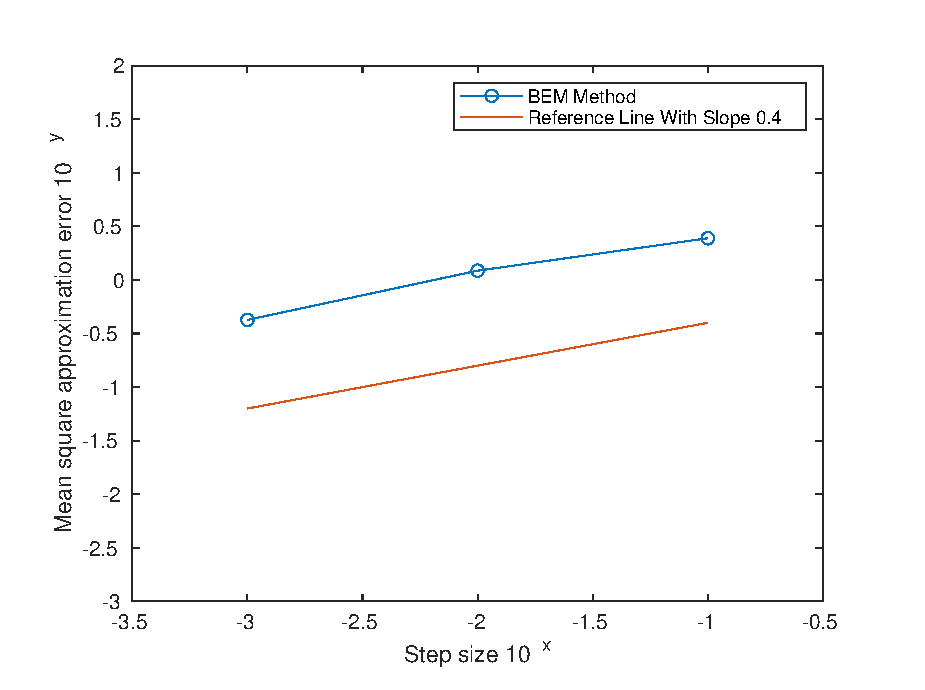
\includegraphics[width=0.45\linewidth]{alpha=0.4.eps}
	\hfill
	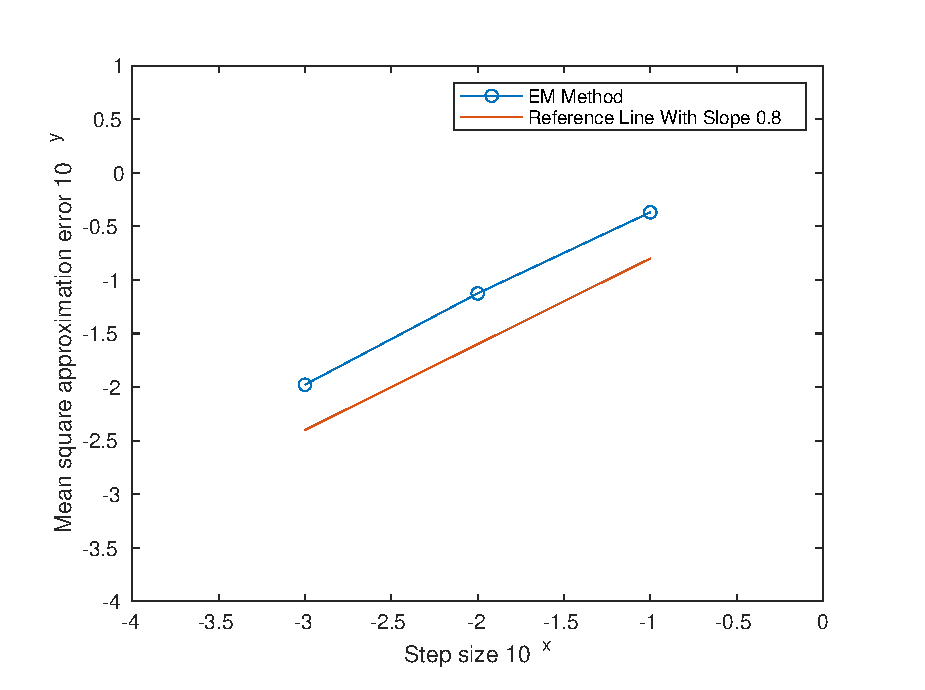
\includegraphics[width=0.45\linewidth]{alpha=0.8.eps}
	\caption{EM方法的$L_1$误差, 左图为$\alpha=0.4$, 右图为$\alpha=0.8$}
	\label{fig:image}
	\vspace{-2ex}
	{}\end{figure}

% 第4章 插图环境

% 微分方程的数值方法

\chapter{BEM数值方法}

\section{假设}

%\begin{assumption}\label{unique}
%	在这一章节中, 我们令$-\infty\leq\alpha<\beta\leq\infty$,并且假设时间变换的SDE\cref{basic SDE}在$(\alpha,\beta)\subseteq\mathbb{R}$有唯一强解,即:$$\mathbb{P}(x(t)\in(\alpha,\beta), t\geq0)=1.$$
%\end{assumption}

	



\begin{assumption}\label{super linear growth}
	在这一章节的中, 我们假设SDE\cref{basic SDE}的漂移项系数$f$满足超线性增长条件, 即存在一个常数$K>0$和$\gamma>1$, 使得
	\begin{equation}
		|f(x)| \le K(1+|x|^{\gamma}). 
	\end{equation}
\end{assumption}

\begin{assumption}\label{momentBEM}
	在这一章节中, 我们假设SDE\cref{basic SDE}的漂移项系数$f$是二阶连续可微的, 并且存在常数$K>0$和$\gamma>1$, 使得
	\begin{equation}
		|f(x)f'(x)| + |\sigma f'(x)| + |\sigma^2 f''(x)| \leq K(1 + |x|^{\gamma}).
	\end{equation}
	
\end{assumption}
对于SDE\cref{basic SDE}在漂移项系数$f$在单调条件下, 解的存在唯一性的证明可以参考\cite{umarov2018beyond}中漂移性满足全局Lipschitz条件的证明.

\section{等距步长的BEM数值方法}

\begin{assumption}\label{monotony}
在这一小节中, 我们令$c\in[-\infty,+\infty),I=(c,+\infty),\operatorname{}d\in I$是区间中任意的一点, 并且假设SDE\cref{basic SDE}的漂移项系数$f$满足下述单调性 :
\begin{equation}
	f:I\to\mathbb{R}  , 使得 \exists K \in\mathbb{R},\forall x,y\in I,x\leq y,f(y)-f(x)\leq K(y-x).
\end{equation}
\end{assumption}

类似与\cref{main pro1}, 我们可以得到下面的命题.
\begin{proposition}\label{main pro2}
	令X是SDE\cref{basic SDE}的解, 其中f满足\cref{monotony}和\cref{super linear growth}, 那么对于任意的$p \ge 1$, 存在常数$c_1,c_1$, 使得$\mathbb{E}_{B}[Y_T^{(p)}] < c_1 e^{c_2E_T }. $, 其中$Y_t^{(p)} := 1 + \sup\limits_{0\le r\le t}|X_r|^p$.
\end{proposition}

对于随机微分方程\cref{basic SDE},它的BEM数值格式是:
\begin{equation}\label{eq:1}
	X_{t_{i+1}}=X_{t_i}+f(X_{t_{i+1}})\Delta E_{i}+\sigma\Delta B_{E_{i}},\quad i=0,1,2,\ldots,\qquad X_0=X(0)
\end{equation}
其中$\Delta E_{i}=E(t_{i+1})-E(t_i)$以及$\Delta B_{E_{i}}=B(E{(t_{i+1})})-B(E({t_i}))$.
\begin{theorem}\label{main th}
	对于任意的常数$\epsilon>0$, 令$\epsilon < T_1 < T_2, \lceil T_1/\Delta t \rceil = m$和$\lceil T_2/\Delta t \rceil = n$, 在 \cref{monotony}, \cref{super linear growth}和\cref{momentBEM}的条件下,存在常数C,使得下面的不等式成立:
	$$\mathbb{E}\left[\sup\limits_{i = m,m+1,\ldots,n} |X({t_i})-X_{t_i}|\right]\le C\Delta t^\alpha.$$
\end{theorem}
\begin{proof}
	由于第一变量变换和第二变量变换公式\cref{first},\cref{second}的成立,使得我们可以考虑\cref{basic SDE}在$[t_i,t_{i+1})$的积分:
	\begin{align}
		\int_{t_i}^{t_{i+1}}dX(s)=\int_{t_i}^{t_{i+1}}f(X(s))dE(s)+\int_{t_i}^{t_{i+1}}\sigma dB(E(s))
	\end{align}
	等价于
	\begin{align}\label{eq:5}
		\int_{t_i}^{t_{i+1}}dX(s))=\int_{E_{t_i}}^{E_{t_{i+1}}}f(X(D(s-)))ds+\int_{E_{t_i}}^{E_{t_{i+1}}}\sigma dB(s)
	\end{align}
	针对于漂移项$f(X(D(s-)))$,下面等式恒成立:
	\begin{align}\label{EMito}
		\int_{E(t_i)}^{E(t_{i+1})} f(X(D(t_{i+1}-)))) - f(X(D(t-))) dt = \int_{E(t_i)}^{E(t_{i+1})} \int^{D(t_{i+1}-)}_{D(t-)} df(X(s)) dt
	\end{align}
	对于$df(X(s))$,由\cref{ito}的时间变换It\^{o}公式:
	\begin{align*}
		\begin{gathered}
			f(X(t))-f(0)=\int_{0}^{E(t)}f(X(D(s-)))f^{\prime}\left(X(D(s-))\right)+\frac{\sigma^{2}}{2}f^{\prime\prime}\big(X(D(s-))\big)ds \\
			+\int_{0}^{E(t)}\sigma f^{\prime}\big(X(D(s-))\big)dB(s)
		\end{gathered}
	\end{align*}
	于是\cref{EMito}变成
	\begin{equation}\label{EMito1}
		\begin{aligned}
			&\quad\int_{E(t_i)}^{E(t_{i+1})} f(X(D(t_{i+1}-))) - f(X(D(t-))) dt \\
			&= \int_{E(t_i)}^{E(t_{i+1})} \int_{t}^{t_{i+1}} \left( f(X(D(s))) f^{\prime}(X(D(s))) + \frac{1}{2} \sigma^2 f^{\prime\prime}(X(D(s))) \right) ds \, dt\\
			&\quad + \int_{E(t_i)}^{E(t_{i+1})} \int_{t}^{t_{i+1}} \sigma f^{\prime}(X(D(s))) \, dB(s) \, dt .
		\end{aligned}
	\end{equation}
	由\cref{eq:5}与\cref{EMito1},以及\cite[Theorem 3.1]{kobayashi2011stochastic}可以得到
	\begin{align*}
		X(t_{i+1}) 
		&= X(t_i) + \int_{E(t_i)}^{E(t_{i+1})} f(X({D(t_{i+1})})) \, dt + \int_{t_i}^{t_{i+1}} \sigma \, dB(E(t)) \\
		&\quad + \int_{E(t_i)}^{E(t_{i+1})} \int_{t}^{t_{i+1}}\left( f(X(D(s))) f^{\prime}(X(D(s))) + \frac{1}{2} \sigma^2 f^{\prime\prime}(X(D(s))) \right) ds \, dt \\
		&\quad + \int_{E(t_i)}^{E(t_{i+1})} \int_{t}^{t_{i+1}}\sigma f^{\prime}(X(D(s)))) \, dB(s) \, dt \\
		&= X(t_i) + \int_{t_i}^{t_{i+1}} f(X({t_i)}) \, dE(t) + \int_{t_i}^{t_{i+1}} \sigma \, dB(E(t)) \\
		&\quad + \int_{t_i}^{t_{i+1}} \int_{E(t)}^{E(t_{i+1})} \left( f(X(D(s))) f^{\prime}(X(D(s))) + \frac{1}{2} \sigma^2 f^{\prime\prime}(X(D(s))) \right) ds \, dE(t) \\
		&\quad + \int_{t_i}^{t_{i+1}} \int_{E(t)}^{E(t_{i+1})}\sigma f^{\prime}(X(D(s))) \, dB(s) \, dE(t)\\
		&= X(t_i) + \int_{t_i}^{t_{i+1}} f(X({t_i})) \, dE(t) + \int_{t_i}^{t_{i+1}} \sigma \, dB(E(t)) \\
		&\quad + \int_{t_i}^{t_{i+1}} \int_{t}^{t_{i+1}} \left( f(X(s)) f^{\prime}(X(s)) + \frac{1}{2} \sigma^2 f^{\prime\prime}(X(s)) \right) dE(s) \, dE(t) \\
		&\quad + \int_{t_i}^{t_{i+1}} \int_{t}^{t_{i+1}}\sigma f^{\prime}(X(s)) \, dB(E(s)) \, dE(t)
	\end{align*}
	因此
	\begin{align}\label{eq:2}
		X(t_{i+1})
		&= X(t_i) + \int_{t_i}^{t_{i+1}} f(X({t_{i+1})}) \, dE(t) + \int_{t_i}^{t_{i+1}} \sigma \, dB(E(t)) + R_i
	\end{align}
	其中
	\begin{align*}
		R_i = &-\int_{t_i}^{t_{i+1}} \int_{t}^{t_{i+1}} \left( f(X(s)) f^{\prime}(X(s)) + \frac{1}{2} \sigma^2 f^{\prime\prime}(X(s)) \right) dE(s) \, dE(t)\\
		&-\int_{t_i}^{t_{i+1}} \int_{t}^{t_{i+1}} \sigma f^{\prime}(X(s)) \, dB(E(s)) \, dE(t)
	\end{align*}
	将$R_i$分解成$R_i = R_i^{(1)} + R_i^{(2)}$,其中:
	\begin{align*}
		& R_s^{(1)} = -\int_{t_i}^{t_{i+1}} \int_{t}^{t_{i+1}} \left( f(X(s)) f^{\prime}(X(s)) + \frac{1}{2} \sigma^2 f^{\prime\prime}(X(s)) \right) dE(s) \, dE(t).\\
		& R_s^{(2)} = -\int_{t_i}^{t_{i+1}} \int_{t}^{t_{i+1}} \sigma f^{\prime}(X(s)) \, dB(E(s)) \, dE(t)  
	\end{align*}
	和离散格式相减,即\cref{eq:2}-\cref{eq:1}得到:
	\begin{equation}
		X({t_{i+1}})-X_{t_{i+1}}=X({t_i})-X_{t_i}+(f{(X({t_{i+1}}))}-f{(X_{t_{i+1}})})\Delta E_{i}+R_{i}
	\end{equation}
	令$e_i = X({t_i})-X_{t_i}$
	由\cref{monotony}得到:
	\begin{equation}
		(1-K_1\Delta E_s)e_{s+1}\leq e(s)+R_{s},\quad\text{其中}s=m,m+1, \ldots ,n
	\end{equation}
	由逆从属过程$E(t)$的Hölder连续性, 即\cref{Einc},可以得到 
	\begin{equation}\label{bound}
	\sup\limits_{k=m,\ldots, n}	\prod\limits_{l=m}^{k}(1-K_1\Delta E_l)^{-1} <\sup\limits_{k=m,\ldots, n}	\prod\limits_{l=m}^{k}(1-C\Delta t^{\gamma})^{-1}
	\end{equation}
	通过对$\Delta t$取极限, 于是
	\[
	\sup\limits_{k=m,\ldots, n}	\prod\limits_{l=m}^{k}(1-K_1\Delta E_l)^{-1}<\infty
	\]
	结合\cref{bound}, 由\cref{gronwall}我们可以得到
	$$\mathbb{E}  \left[\sup\limits_{k=m,\ldots, n}|e_k|\right] \leq C\mathbb{E}\sum\limits_{j=m}^{n}\left|R_{j}^{(1)} \right| + C\mathbb{E}\sum\limits_{j=m}^{n}\left|R_{j}^{(2)} \right|.$$
	
	对于第一项,  由\cref{momentBEM}, \cref{main pro2}和\cref{boundE}, 可以得到
	\begin{align*}
		\mathbb{E} \left[|R_{j+1}^{(1)}| \right] &= \mathbb{E}_D \left[
		\int_{t_i}^{t_{i+1}} \int_{t_i}^{t}  \mathbb{E}_B \left( f(X(s)) f^{\prime}(X(s)) + \frac{1}{2} \sigma^2 f^{\prime\prime}(X(s)) \right) dE(s) \, dE(t)
		\right] \\
		&= C\mathbb{E}_D \left[
		\int_{t_i}^{t_{i+1}} \int_{t_i}^{t}  \mathbb{E}_B \left[1+|X(s)|^{\gamma} \right] dE(s) \, dE(t)
		\right] \\
		& \le C\mathbb{E}_D \left[
		\int_{t_i}^{t_{i+1}} \int_{t_i}^{t}  e^{\gamma E(s)} dE(s) \, dE(t)
		\right] \\
		& \le C\mathbb{E}_D \left[
		\int_{t_i}^{t_{i+1}} \int_{t_i}^{t}  e^{\gamma T} dE(s) \, dE(t)
		\right] \\
		&\le C\Delta t^{1+\alpha}. 
	\end{align*}
	于是
	\begin{equation}
		\sum\limits_{m}^{n}\mathbb{E}\left|R_{j}^{(1)}\right| \leq
		C\sum\limits_{j=m}^{n}\Delta t^{1+\alpha} \le C\Delta t^\alpha
	\end{equation}
	因为
	\begin{align*}
		\mathbb{E}\left[ R_{k}^{(2)}|\mathcal{F}_{k\Delta t} \right] &= \mathbb{E}_D\mathbb{E}_B\left[ \int_{t_i}^{t_{i+1}} \int_{t_i}^{t} \sigma f^{\prime}(X(s)) \, dB(E(s)) \, dE(t) \right]\\
		&=\mathbb{E}_D\left[ \int_{t_i}^{t_{i+1}} \mathbb{E}_B\int_{t_i}^{t} \sigma f^{\prime}(X(s)) \, dB(E(s)) \, dE(t) \right]\\
		&= 0
	\end{align*}
	因此
	\begin{align*}
		\sum_{j=m}^{n}R_{j}^{(2)} 
	\end{align*}
	是鞅.我们知道由BDG不等式和\cref{main lemma}可以得到:
	\begin{equation*}
		\mathbb{E}[dB_EdE]^2=\mathbb{E}[(dB_E)^2(dE)^2]=\mathbb{E}_D[(dE)^2\mathbb{E}_B(dB_E)^2]\leq
		C\mathbb{E}_{D}[dE]^3\leq C\Delta t ^{1+2\alpha}
	\end{equation*}
	于是对于第二项, 
	\begin{align*}
		\mathbb{E} \left[|R_{j+1}^{(2)}| \right] &= \mathbb{E}_D \left[
		\int_{t_i}^{t_{i+1}} \mathbb{E}_B  \left[\int_{t_i}^{t}  \sigma f^{\prime}(X(s)) dB_{E(s)}\right] \, dE(t)
		\right] \\
		& \le C\mathbb{E}_D \left[
		\int_{t_i}^{t_{i+1}} \left[\int_{t_i}^{t}  \mathbb{E}_B\left(\sigma f^{\prime}(X(s))\right)^2 dE(s)\right]^{\frac{1}{2}} \, dE(t)
		\right] \\
		&\le C \mathbb{E}_D 
		\int_{t_i}^{t_{i+1}} \left[\int_{t_i}^{t}  1 dE(s)\right]^{\frac{1}{2}} \, dE(t)\\
		&\le C\Delta t^{\frac{1}{2}+\alpha}. 
	\end{align*}
	
	由BDG不等式和Cauchy-Schwarz不等式,可以得到:
	\begin{equation*}
		\mathbb{E}\sum_{j=m}^{n}\left|R_{j}^{(2)}\right|  \le C\mathbb{E} \left|\sum_{j=m}^{n}(R_{j}^{(2)})^2\right|^{\frac{1}{2}} \le C\sqrt{\sum_{j=m}^{n}\mathbb{E}(R_{j}^{(2)})^2}
		\le C\sqrt{\sum_{j=m}^{n}\Delta t^{1+2\alpha}} \le C\Delta t^{\alpha}
	\end{equation*}
	综上所述,
	\begin{equation*}
		\mathbb{E} [e_n] \leq C\Delta t^\alpha
	\end{equation*}
\end{proof}
%	tips:We have also proved that $\mathbb{E} [\Delta E \Delta B_E ] \le C\Delta t ^{1+\frac{\alpha}{2}}$,however it seems that it's nothing help here.


\section{随机步长的BEM数值方法}

\begin{assumption}\label{Local Lipschitz}
	在这一小节中, 我们假设SDE\cref{basic SDE}的漂移项系数$f$满足单边Lipschitz, 即存在常数$K>0$使得
	\begin{equation}
		(x-y)(f(x)-f(y)) \le K|x-y|^2
	\end{equation}
\end{assumption}

类似与 \textnormal{\cref{nostostep}}和\textnormal{\cref{intX}},
我们可以得到对应的BEM数值格式.
\begin{equation}\label{nostostepY}
	X_{\tau_{n+1}} :=X_{\tau_n}  + f\left(X_{\tau_{n+1}}\right)\delta + \sigma\left(B_{(n+1)\delta}-B_{n\delta}\right).
\end{equation}

\begin{equation}\label{intY}
	X_s:= X_{\tau_n} +  \int_{\tau_n}^s f\left(X_{\tau_{n+1}}\right) \, dE_r + \int_{\tau_n}^s \sigma dB_{E_r}.
\end{equation}

%\begin{theorem}
%	设 $X$ 为随机微分方程 (3.1) 的解,假设条件 $\mathcal{H}_1, \mathcal{H}_2$ 和 $\mathcal{H}_4$ 满足。
%	设 $X^{\delta}$ 为在 (4.3)–(4.4) 中定义的 Euler-Maruyama 型近似过程。则存在与 $\delta$ 无关的常数 $C > 0$,使得对所有 $\delta \in (0,1)$,
%	\[
%	\mathbb{E} \left[ \sup_{0 \leq s \leq T} | X_s - X_s^\delta | \right] \leq C \delta。
%	\]
%	因此,$X^\delta$ 在 $[0, T]$ 上以 1 阶一致强收敛于 $X$。
%\end{theorem}

\begin{theorem}\label{main th BEM1}
	设 $X$ 为SDE\textnormal{\cref{basic SDE} }的解,在 \textnormal{\cref{super linear growth}}, \textnormal{\cref{momentBEM}}和\textnormal{\cref{Local Lipschitz}}的条件下, 
	设 $X_t$ 为在 \textnormal{\cref{nostostepY}}和\textnormal{\cref{intY}}中定义的BEM数值方法。则存在与 $\delta$ 无关的常数 $C > 0$,使得对所有 $\delta \in (0,1)$,
	\[
	\mathbb{E} \left[ \sup_{0 \leq s \leq T} | X(s) - X_s | \right] \leq C \delta。
	\]
	因此,$X_t$ 在 $[0, T]$ 上以 1 阶一致强收敛于 $X(t)$。
\end{theorem}

-----------------------------------------------------------------------------------------

\begin{proof}
	
	利用 (3.1) 并通过 Itô 公式展开 $\mathrm{d}E_r$ 积分的被积函数,
	
	$$
	\begin{aligned}
		X_{\tau_{n+1}} &= X_{\tau_n} +  \int_{\tau_n}^{\tau_{n+1}} f(X_{\tau_n}) \, \mathrm{d}E_r + \int_{\tau_n}^{\tau_{n+1}} \sigma \, \mathrm{d}B_{E_r} + R_{(\tau_n, \tau_{n+1})}; \\
		R_{(a,b)} &:=  \int_a^b \int_a^{r_2} \left( f(X_{\tau_{n_{r_1}}})f'(X_{\tau_{n_{r_1}}}) + \frac{\sigma ^2}{2} f''(X_{\tau_{n_{r_1}}})  \right) \, \mathrm{d}E_{r_1} \, \mathrm{d}E_{r_2} + \int_a^b \int_a^{r_2} \sigma f'(X_{\tau_{n_{r_1}}})   \, \mathrm{d}B_{E_{r_1}} \, \mathrm{d}E_{r_2},
	\end{aligned}
	$$
	因此:
	$Z_t := \sup_{0 \leq s \leq t} | X_s - {X_s^\delta} | \leq I_1 + I_2 $,其中
	
	$$
	\begin{aligned}
		&I_1 := \sup_{0 \leq s \leq t} \left| \int_0^s F(X_{\tau_{n_r}}) - F(X_{\tau_{n_r}}^\delta)  \, \mathrm{d}E_r \right|; \\
		&I_2 := \sup_{0 \leq s \leq t} \left| \sum_{i=0}^{n_s - 1} R_{(\tau_{t}, \tau_{t+1})} + R_{(\tau_{n_s}, s)} \right|.
	\end{aligned}
	$$
	很容易观察到
	\begin{equation}\label{II1}
		\mathbb{E}_B[I_1] \leq C \int_0^t \mathbb{E}_B[Z_r] \, \mathrm{d}E_r.
	\end{equation}
	
	主要的技术部分涉及余项 $I_2$,其中包含两个不同的双重积分:$\mathrm{d}E_{r_1} \, \mathrm{d}E_{r_2}$ 和 $\mathrm{d}B_{E_{r_1}} \, \mathrm{d}E_{r_2}$。我们将在下面逐一处理这些积分。
	
	对于第一个积分$ \mathrm{d}E_{r_1} \, \mathrm{d}E_{r_2}$,
	\begin{align}
		& \quad \mathbb{E}_B \left[\sup_{0 \leq s \leq t} \left| \int_0^s \int_{\tau_{n_2}}^{r_2} ff'  + \frac{\sigma^2}{2} f'' \, \mathrm{d}E_{r_1} \, \mathrm{d}E_{r_2} \right|\right] \nonumber \\
		&\leq  \frac{3}{2}K \mathbb{E}_B[Y_T^{(1)}] \int_0^t \int_{\tau_{n_{r_2}}}^{r_2} \, \mathrm{d}E_{r_1} \, \mathrm{d}E_{r_2} \nonumber \\
		&\leq  \frac{3}{2}K E_T \mathbb{E}_B[Y_T^{(1)}] \delta.  \label{II21}
	\end{align}
	
	另一方面,我们需要估计 $\mathbb{E}_B \left[\sup_{0 \leq s \leq t} |M_{n_s} + U_s|\right]$,其中 $M_0 := 0$,对于 $n \geq 1$,$M_n := \sum_{i=0}^{n-1} L_i$,
	$$
	L_i := \int_{\tau_i}^{\tau_{i+1}} \int_{\tau_i}^{r_2} \sigma f' \, \mathrm{d}B_{E_{r_1}} \, \mathrm{d}E_{r_2}, \quad U_s := \int_{\tau_{n_s}}^s \int_{\tau_{n_s}}^{r_2} \sigma f' \, \mathrm{d}B_{E_{r_1}} \, \mathrm{d}E_{r_2}.
	$$
	
	我们首先验证随机积分 $L_i, i=0,1,\ldots,n_t-1$ 关于 $\mathbb{P}_B$ 是不相关的。令 $i < j$,因此 $\tau_{i+1} \leq \tau_j$。观察到 $\mathbb{E}_B [L_i L_j] = \mathbb{E}_B \left[L_i \mathbb{E}_B [L_j | \mathcal{F}_{E_{\tau_j}}]\right]$。根据假设和估计 (3.4),
	
	$$
	\mathbb{E}_B \left[\int_{\tau_j}^{\tau_{j+1}} \left|\int_{\tau_j}^{r_2} F_x G( X_{r_1}) \, \mathrm{d}B_{E_{r_1}}\right|^2 \mathrm{d}E_{r_2}\right] \leq \delta^2 K^2 \mathbb{E}_B [Y_t^{(2)}] < \infty.
	$$
	
	因此,$\mathbb{E}_B \left[L_j | \mathcal{F}_{E_{\tau_j}}\right] = \int_{\tau_j}^{\tau_{j+1}} \mathbb{E}_B \left[\int_{\tau_j}^{r_2} F_x G(X_{r_1}) \, \mathrm{d}B_{E_{r_1}} | \mathcal{F}_{E_{\tau_j}}\right] \mathrm{d}E_{r_2} = 0$,这是由于条件 Fubini 定理(参考文献 [26] 中的定理 27.17)和鞅性质,从而得到不相关性。另一方面,由于 $E$ 具有连续路径,变量变换公式(参考文献 [13] 中的定理 3.1)表明 $M_n$ 可以表示为
	
	$$
	\sum_{i=0}^{n-1} \int_{i\delta}^{(i+1)\delta} \int_{i\delta}^{E_{r_2}} \sigma f' \, \mathrm{d}B_{r_1} \, \mathrm{d}r_2。
	$$
	
	该表示式,以及参考文献 [12] 中引理 5.7.1 和 10.8.1 的证明,表明离散时间过程 $(M_n)_{n \geq 0}$ 是一个平方可积的 $((\mathcal{F}_{n\delta})_{n \geq 0}, \mathbb{P}_B)$-鞅,初始值为 0。因此,由 BDG 不等式 (3.2) 和 $L_i$ 的不相关性,
	
	$$
	\mathbb{E}_B \left[\sup_{0 \leq s \leq t} M_{n_s}^2\right] \leq b_2 \sum_{i=0}^{n_t-1} \mathbb{E}_B [L_i^2]。
	$$
	因此,由 Cauchy-Schwartz 不等式,
	\begin{align}
		\mathbb{E}_B\left[\sup_{0\leq s\leq t}M_{n_s}^2\right] 
		&\leq b_2\delta\sum_{i=0}^{n_t-1}\int_{\tau_i}^{\tau_{i+1}}\mathbb{E}_B
		\left[\int_{\tau_i}^{r_2}\left|\sigma f'\right|^2\mathrm{d}E_{r_1}\right]
		\mathrm{d}E_{r_2} \nonumber \\
		&\leq2b_2\delta K^2\mathbb{E}_B[Y_T^{(2)}]\sum_{i=0}^{n_t-1}\int_{\tau_i}^
		{\tau_{i+1}}(E_{r_2}-E_{\tau_i})\mathrm{d}E_{r_2} \nonumber \\
		&\leq 2b_2E_TK^2\mathbb{E}_B[Y_T^{(2)}]\delta^2. \label{II221}
	\end{align}
	另一方面, 
	\begin{align}
		\mathbb{E}_B\left[\sup_{0\leq s\leq t}U_s^2\right]  
		&\leq\mathbb{E}_B\biggl[\sup_{0\leq s\leq t}(E_s-E_{\tau_{n_s}})\int_{\tau_{n_s}}^s\left|\int_{\tau_{n_s}}^{r_2}\sigma f'\mathrm{d}B_{E_{r_1}}\right|^2\mathrm{d}E_{r_2}\biggr] \nonumber \\ &\leq\delta\int_0^t\mathbb{E}_B\left[\sup_{s\in[r_2,t]}\left|\int_{\tau_{n_s}}^{r_2}\sigma f'\mathrm{d}B_{E_{r_1}}\right|^2\right]\mathrm{d}E_{r_2}.\label{II222}
	\end{align}
	由于$\{(\tau_{n_s},r_2)~:~r_2~\leq~s~\leq~t\}~\subset~\{(\tau_{n_{r_2}},u)~:~\tau_{n_{r_2}}~\leq~u~\leq~r_2\},$于是
	\begin{align*}
		&\quad\mathbb{E}_B\Big[\sup_{S\in[r_2,t]}\Big|\int_{\tau_x}^{r_2}\sigma f'\mathrm{d}B_{E_{r_1}}\Big|^2\Big]  \\
		&\le \mathbb{E}_B\left[\sup_{u\in[\tau_{n_{r_2}},r_2]}\left|\int_{\tau_{n_{r_2}}}^u\sigma f'\mathrm{d}B_{E_{r_1}}\right|^2\right] \\
		&\leq b_2\mathbb{E}_B\left[\int_{\tau_{n_{r_2}}}^{r_2}\left|\sigma f'\right|^2\mathrm{d}E_{r_1}\right]\\
		&\leq 2b_2K^2\mathbb{E}_B[Y_T^{(2)}]\delta.
	\end{align*}
	因此,\cref{II222}的上界为  $2b_2E_TK^2\mathbb{E}_B[Y_T^{(2)}]\delta^2.$ 将其与 \cref{II221} 结合得:
	\begin{equation}\label{II22}
		\mathbb{E}_B\left[\sup_{0\leq s\leq t}|M_{n_s}+U_s|^2\right] 
		\leq 8b_2E_TK^2\mathbb{E}_B[Y_T^{(2)}]\delta^2. 
	\end{equation}
	根据估计 \cref{II21} 和 \cref{II22},
	\begin{equation}\label{II2}
		\mathbb{E}_B[I_2] 
		\leq \left\{\frac{3}{2}E_T\mathbb{E}_B[Y_T^{(1)}]+(8b_2E_T\mathbb{E}_B[Y_T^{(2)}])^{1/2}\right\}K\delta. 
	\end{equation}
	
	现在,将 \cref{II1}和 \cref{II2}与  $\mathbb{E}_B[Y_T^{(1)}]\leq\sqrt{2}\mathbb{E}_B[Y_T^{(2)}]^{1/2}$ 结合得:
	\begin{equation*}
		\mathbb{E}_B[Z_t] 
		\leq \xi_2(E_T)\mathbb{E}_B[Y_T^{(2)}]^{1/2}\delta + K\int_0^t\mathbb{E}_B[Z_r] \mathrm{d}E_r.
	\end{equation*}
	
	其中 $\xi_2(u) := K(\frac{3\sqrt{2}}{2}u + (8b_2u)^{1/2}).$
	应用 Gronwall 类型不等式, 对两边取 $ \mathbb{E}_D $并使用 Cauchy-Schwartz 不等式得 
	\begin{equation*}
		\mathbb{E}[Z_T] \leq \mathbb{E}[\xi_2^4(E_T)]^{1/4}\mathbb{E}[(Y_T^{(2)})^2]^{1/4}\mathbb{E}[e^{2KE_T}]^{1/2}\delta.
	\end{equation*}
	由于对于任意的$\lambda>0, t>0,n>0$, 都有$\mathbb{E}[e^{\lambda E_t}] < \infty$, 以及$\mathbb{E}[E^n(t)] < \infty$, 再结合\cref{main pro1}, 于是可以得到该定理成立.
	
	
	\section{数值模拟}
	
	\begin{example}
		考虑时间变换的的布朗运动驱动的CIR过程
		\begin{equation}\label{CIR}
			dy(t)=\kappa(\theta-y(t))dE(t)+\sigma\sqrt{y(t)}dB(E(t)),\quad t\geq0,\quad y(0)>0.
		\end{equation}
	\end{example}
	如果 $2\kappa\theta\geq\sigma^{2}$, 那么 $D=(0,\infty)$ 并且\cref{unique} 在 $(\alpha,\beta)=$
	$(0,\infty)$是成立的. 
	另外, 使用It\^{o}公式$X(t)=F((y(t))$,其中$F$是由\cref{Lamperti}定义,即对时间变换的CIR过程进行Lamperti变换可以得到
	\begin{equation}
		dX(t)=f(X(t))dE(t)+\frac12\sigma dB(E(t)),\quad t\geq0,\quad X(0)=\sqrt{y(0)}
	\end{equation}
	其中
	\begin{equation}
		f(X)=\dfrac{1}{2}\kappa\left(\theta_vX^{-1}-X\right),\quad X>0
	\end{equation}
	其中 $\theta_v=\theta-\frac{\sigma^2}{4\kappa}$ ,并且 BEM数值格式如下
	\begin{equation}
		X_{t_{i+1}}=X_{t_{i}}+f(X_{t_{i+1}})\Delta E_i+\frac{1}{2}\sigma\Delta B_{E_i},\quad k=0,1,\dots 
	\end{equation}
	观察到
	\begin{equation}
		f'(X)=-\frac{1}{2}\kappa(\theta_vX^{-2}+1)
	\end{equation}
	以及
	\begin{equation}
		f(X)f'(X)+\frac{\sigma^2}{2}f''(X)=-\frac{\kappa^2}{4}(\theta_v^2X^{-3}-X)+\frac{1}{2}\kappa\theta_vX^{-3}\sigma^2.
	\end{equation}
	因此为了满足\cref{moment},只需要满足
	\begin{equation}
		\sup_{0\leq t\leq T}\mathbb{E}[X(t)^{-3}]=\sup_{0\leq t\leq T}\mathbb{E}[y(t)^{-\frac{3}{2}}] < \infty.
	\end{equation}
	对于时间变换的CIR过程y(t)的矩有界,即
	\begin{equation}
		\sup\limits_{0\leq t\leq T}\mathbb{E}[y(t)^q]<\infty\quad\mathrm{for}\quad q>-\frac{2k\theta}{\sigma^2},
	\end{equation}
	下面验证,对于由时间变换的的布朗运动驱动的CIR过程\cref{CIR}的精确解矩有界.
	\begin{proposition}
		对于由时间变换的布朗运动驱动的CIR过程\cref{CIR},其中$y_0>0$,$1<p<\frac{2K\theta}{\sigma^2}-1$,都存在一个常数C使得
		\begin{equation*}
			\sup\limits_{t\in[0,T]}\mathbb{E}\left[\left(y(t)\right)^{-p}\right]\leq C(1+y(0)^{-p})
		\end{equation*}
	\end{proposition}
	\begin{proof}
		定义停时$\tau_{n}=\mathrm{inf}\{0<s\leq T;y(s)\leq1/n\}$,通过It\^{o}公式,我们可以得到
		$$\begin{aligned}
			\mathbb{E}_B\left[(y(t\wedge\tau_{n}))^{-p}\right] &=y(0)^{-p}-p\mathbb{E}_B\left[\int_{0}^{t\wedge\tau_{n}}\frac{K(\theta-y(s))}{(y(s))^{p+1}}dE(s)\right]\\
			&+p(p+1)\frac{\sigma^{2}}{2}\mathbb{E}_B\left[\int_{0}^{t\wedge\tau_{n}}\frac{1}{(y(s))^{p+1}}dE(s)\right] \\
			&\leq y(0)^{-p}+pK\int_{0}^{t}\mathbb{E}_B\left(\frac{1}{(y(s\wedge\tau_{n}))^{p}}
			\right)dE(s) \\
			&+\mathbb{E}_B\left[\int_0^{t\wedge\tau_n}\frac{p\left(\frac{(p+1)\sigma^2}{2}-K\theta\right)}{(y(s))^{p+1}}dE(s)\right]
		\end{aligned}$$
		通过计算可以找到正数$\underline C$使得, 当$\frac{(p+1)\sigma^2}{2}-K\theta<0$时,对于任意的 $y(0)=x>0$,都有
		$$\frac{p\left(\frac{(p+1)\sigma^2}{2}-K\theta\right)}{x^{p+1}}\leq \underline C$$
		因此
		$$\mathbb{E}_B\left[(y(t\wedge\tau_n))^{-p}\right]\leq y(0)^{-p}+\underline{C}E(T)+pK\int_0^t\sup_{r\in[0,s]}\mathbb{E}_B\left[(y(r\wedge\tau_n))^{-p}\right]dE(s)$$
		于是由Gronwall不等式,可以得到
		$$\sup\limits_{t\in[0,T]}\mathbb{E}_B\left[(y(t\wedge\tau_n)^x)^{-p}\right]\leq\left(y(0)^{-p}+\underline{C}E(T)\right)\exp(pKE(T))$$
		两边同时取$\mathbb{E}_D$并使用Cauchy-Schwarz不等式,得到
		$$\begin{aligned}
			\sup\limits_{t\in[0,T]}\mathbb{E}\left[(y(t\wedge\tau_n)^x)^{-p}\right]&\leq\mathbb{E}\left[\left(y(0)^{-p}+\underline{C}E(T)\right)\exp(pKE(T))\right]\\
			&\leq\sqrt{\mathbb{E}\left[\left(y(0)^{-p}+\underline{C}E(T)\right)^2\right]\mathbb{E}\left[\exp(2pKE(T))\right]}
		\end{aligned}$$
		从\cite{jum2014strong}可以得到
		\begin{equation}
			\mathbb{E}[E^n(t)]=\frac{n!}{\Gamma(n\alpha+1)}t^{n\alpha}
		\end{equation}
		\begin{equation}
			\mathbb{E}[e^{\lambda E(t)}]<\infty
		\end{equation}
		其中$\lambda \in \mathbb{R},t>0$.最后,让 $n\to+\infty$,我们完成了这个证明.
	\end{proof}
	\begin{remark}
		在这里只是证明了当$1<p<\frac{2K\theta}{\sigma^2}-1$的时候,矩的存在性,实际上更可以证明$p<\frac{2K\theta}{\sigma^2}$,但是证明起来过于复杂,这里就不在说明,对于我们的结果已经够用了.
	\end{remark}
	对于\cref{moment},可以验证只需要保证$1 < \frac{4}{3}\frac{k\theta}{\sigma^2}$成立即可,而这个区间可以被$1<p<\frac{2K\theta}{\sigma^2}-1$包含在内,因此只需要保证p在后者这个区间即可.至于\cref{monotony},在$(0,\infty)$中很容易可以验证存在这样的$\kappa$使之成立.因此由\cref{main th}可以得到,对于时间变换的CIR过程,使用BEM数值格式的强收敛阶是$\alpha$.
	
	在我们的数值实验中,我们关注端点$T = 1$处的$L_1$误差,因此我们令
	\begin{align*}
		e_T^{i}=\mathbb{E}\left|X_T^{\delta _{15}}-X_T^{\delta _i}\right|
	\end{align*}
	其中$X_T^{\delta _i}$是步长为$\delta _i$时T处的模拟值,$\delta _i = 2^{-i}$,对于我们的数值实验,取$\theta=0.125,\kappa=2$以及$\sigma=0.5$,采用蒙德卡洛方法,
	\begin{align*}
		e_{T}^i\approx\frac{1}{10^3}\sum_{j=1}^{10^3}\left|X_T^{\delta _{15}}-X_T^{\delta _i}\right|.
	\end{align*}
	选择步长为$2^{-15}$作为参考,通过${2^{-11},2^{-10},2^{-9},2^{-8}}$的步长来估计$L_1$误差.
	
	\begin{example}
		考虑时间变换的的布朗运动驱动的CEV过程
		\begin{equation}\label{CEV}
			dy(t)=\kappa(\theta-y(t))dE(t)+\sigma y(t)^\alpha dB_{E(t)}
		\end{equation}
	\end{example}
	
	其中 $0.5<\alpha<1,\kappa,\theta,\sigma>0.$ 通过变换$X(t)=F(y(t))$的变换之后,其中$F$是由\cref{Lamperti}定义,我们可以得到\cref{monotony}在$(\alpha,\beta)=(0,\infty)$下,是成立的,此时	$$dX(t)=f(X(t))dE(t)+(1-\alpha)\sigma dB(E(t))$$
	其中
	$$f(X)=(1-\alpha)\left(\kappa\theta X^{-\frac\alpha{1-\alpha}}-\kappa X-\frac{\alpha\sigma^2}2X^{-1}\right),\quad X>0.$$
	同时我们需要验证另一个\cref{moment}.因为 $\alpha>0.5$, 于是$\frac{1}{1-\alpha}>2$,因此
	$$f^{\prime}(X)=-\alpha\kappa\theta X^{-\frac1{1-\alpha}}-(1-\alpha)\kappa+(1-\alpha)\frac{\alpha\sigma^2}2X^{-2},\quad X>0$$
	同时我们又有
	$$f^{\prime\prime}(X)=\frac\alpha{1-\alpha}\kappa\theta X^{-\frac{2-\alpha}{1-\alpha}}-(1-\alpha)\alpha\sigma^2X^{-3}.$$
	下面验证,对于由时间变换的的布朗运动驱动的CEV过程\cref{CEV}的精确解矩有界.
	\begin{proposition}
		对于由时间变换的布朗运动驱动的CEV过程\cref{CEV},其中$X_0>0$,对于任意的$\frac{1}{2}<\alpha<1$和任意的$p>0$,都存在一个常数C使得
		\begin{equation*}
			\sup\limits_{t\in[0,T]}\mathbb{E}\left[\left(y(t)\right)^{-p}\right]\leq C(1+y(0)^{-p})
		\end{equation*}
	\end{proposition}
	\begin{proof}
		定义停时$\tau_{n}=\mathrm{inf}\{0<s\leq T;y(s)\leq1/n\}$,通过It\^{o}公式,我们可以得到
		$$\begin{aligned}
			\mathbb{E}_B\left[(y(t\wedge\tau_{n}))^{-p}\right] &=y(0)^{-p}-p\mathbb{E}_B\left[\int_{0}^{t\wedge\tau_{n}}\frac{K(\theta-y(s))}{(y(s))^{p+1}}dE(s)\right]\\
			&+p(p+1)\frac{\sigma^{2}}{2}\mathbb{E}_B\left[\int_{0}^{t\wedge\tau_{n}}\frac{1}{(y(s))^{p+2(1-\alpha)}}dE(s)\right] \\
			&\leq y(0)^{-p}+pK\int_{0}^{t}\mathbb{E}_B\left(\frac{1}{(y(s\wedge\tau_{n}))^{p}}
			\right)dE(s) \\
			&+\mathbb{E}_B\left[\int_0^{t\wedge\tau_n}\left(p(p+1)\frac{\sigma^2}{2}\frac{1}{(y(s))^{p+2(1-\alpha)}}-p\frac{K\theta}{(y(s))^{p+1}}\right)dE(s)\right]
		\end{aligned}$$
		可以找到正数$C$使得, 对于任意的 $y(0)=x>0$,都有
		$$\left(p(p+1)\frac{\sigma^2}{2}\frac{1}{x^{p+2(1-\alpha)}}-p\frac{K\theta}{x^{p+1}}\right)\leq C$$
		通过计算可以得到,$\underline C=p(2\alpha-1)\frac{\sigma^2}{2}\left[(p+2(1-\alpha))\frac{\sigma^2}{2K\theta}\right]^{\frac{p+2(1-\alpha)}{2\alpha-1}}$ 是最小的上界. 因此
		$$\mathbb{E}_B\left[(y(t\wedge\tau_n))^{-p}\right]\leq y(0)^{-p}+\underline{C}E(T)+pK\int_0^t\sup_{r\in[0,s]}\mathbb{E}_B\left[(y(r\wedge\tau_n))^{-p}\right]dE(s)$$
		于是由Gronwall不等式,可以得到
		$$\sup\limits_{t\in[0,T]}\mathbb{E}_B\left[(y(t\wedge\tau_n)^x)^{-p}\right]\leq\left(y(0)^{-p}+\underline{C}E(T)\right)\exp(pKE(T))$$
		两边同时取$\mathbb{E}_D$并使用Cauchy-Schwarz不等式,得到
		$$\begin{aligned}
			\sup\limits_{t\in[0,T]}\mathbb{E}\left[(y(t\wedge\tau_n)^x)^{-p}\right]&\leq\mathbb{E}\left[\left(y(0)^{-p}+\underline{C}E(T)\right)\exp(pKE(T))\right]\\
			&\leq\sqrt{\mathbb{E}\left[\left(y(0)^{-p}+\underline{C}E(T)\right)^2\right]\mathbb{E}\left[\exp(2pKE(T))\right]}
		\end{aligned}$$
		从\cite{jum2014strong}可以得到
		\begin{equation}
			\mathbb{E}[E^n(t)]=\frac{n!}{\Gamma(n\alpha+1)}t^{n\alpha}
		\end{equation}
		\begin{equation}
			\mathbb{E}[e^{\lambda E(t)}]<\infty
		\end{equation}
		其中$\lambda \in \mathbb{R},t>0$.最后,让 $n\to+\infty$,我们完成了这个证明.
	\end{proof}
	
	
	由Lamperti变换可知,$X(t)$的逆阶矩可以$y(t)$的逆阶矩控制,于是\cref{moment}成立.因此根据\cref{main th}可以得到由时间变换布朗运动驱动的CEV过程的收敛阶是$\alpha$
	\
	
	\begin{figure}[htp!]
		\centering
		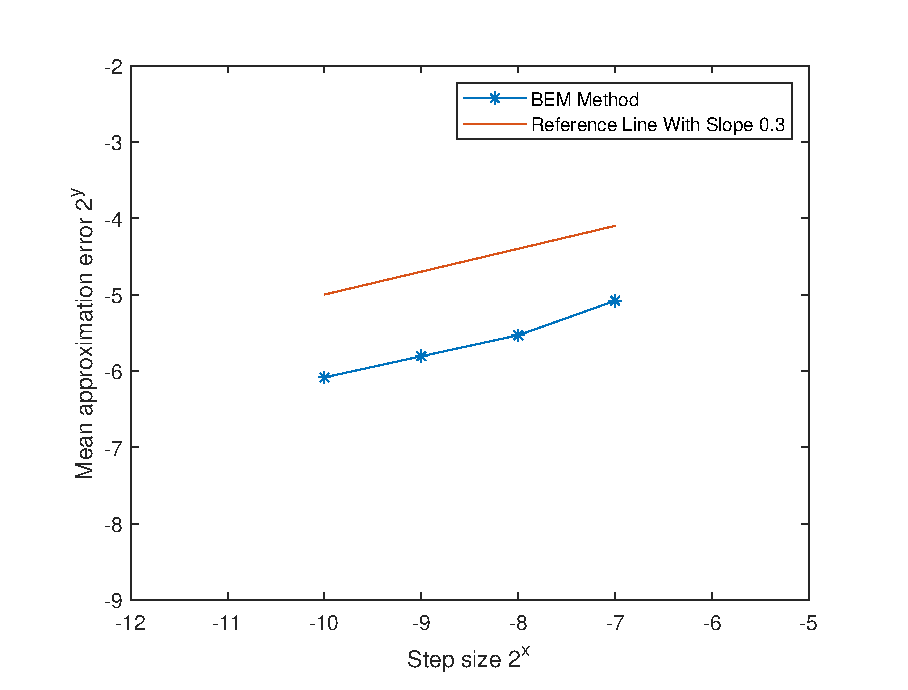
\includegraphics[width=0.45\linewidth]{BEMalpha=0.3.eps}
		\hfill
		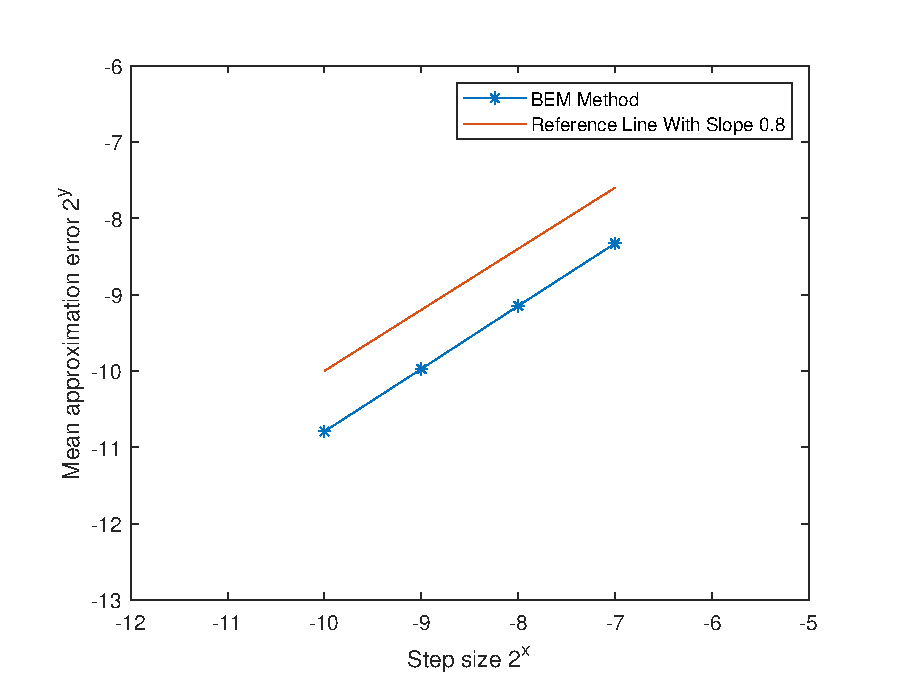
\includegraphics[width=0.45\linewidth]{BEMalpha=0.8.eps}
		\caption{时间变换CIR过程的数值解与解析解之间的绝对误差估计.左图是$\alpha=0.3$,右图是$\alpha=0.8$}
		\label{fig:image}
		\vspace{-2ex}
	\end{figure}
	
	
	
	
\end{proof}

% 第5章 表格环境

% 表格环境

\chapter{结论与展望}




%============== 参考文献 ==============%

% 生成参考文献, 两种方式任选一种

% 第一种方式, 使用 bib 文件
%\nocite{*}  % 可以显示全部参考文献
\bibliography{refs}

%------------------------------------%

% 第二种方式, 手动添加文献信息
%
% 手动添加参考文献

\begin{thebibliography}{99}
\bibitem{Tadmor2012} Tadmor~E. A review of numerical methods for nonlinear partial differential equations\allowbreak[J]. Bull. Amer. Math. Soc., 2012, 49(4): 507-554.

\bibitem{LiLiu1997} 李荣华, 刘播. 微分方程数值解法\allowbreak[M]. 第四版. 北京: 高等教育出版社, 2009.

\bibitem{Adams2003} Adams~R~A, Fournier~J~J~F. Sobolev spaces\allowbreak[M]. 2nd ed. Amsterdam: Elsevier, 2003.

\bibitem{TreWei2014}Trefethen~L~N, Weideman~J~A~C. The exponentially convergent trapezoidal rule\allowbreak[J]. SIAM Rev., 2014, 56(3): 385-458.

\bibitem{Shen1994} Shen~J. Efficient spectral-Galerkin method I. Direct solvers of second- and fourth-order equations using Legendre polynomials\allowbreak[J]. SIAM J. Sci. Comput., 1994, 15(6): 1489-1505.

\end{thebibliography}



%=============== 附录 ================%

% 添加附录, 如不需要可以注释
%
% 附录

\appendix

% 附录正文
\chapter{这是第一个附录}

\section{附录A的小节}

这里是附录环境.

附录公式及编号
\begin{equation}\label{eq:abc}
  a^2+b^2=c^2.
\end{equation}

如图~\ref{fig:sinx2}.
\begin{figure}[htp!]
  \centering
  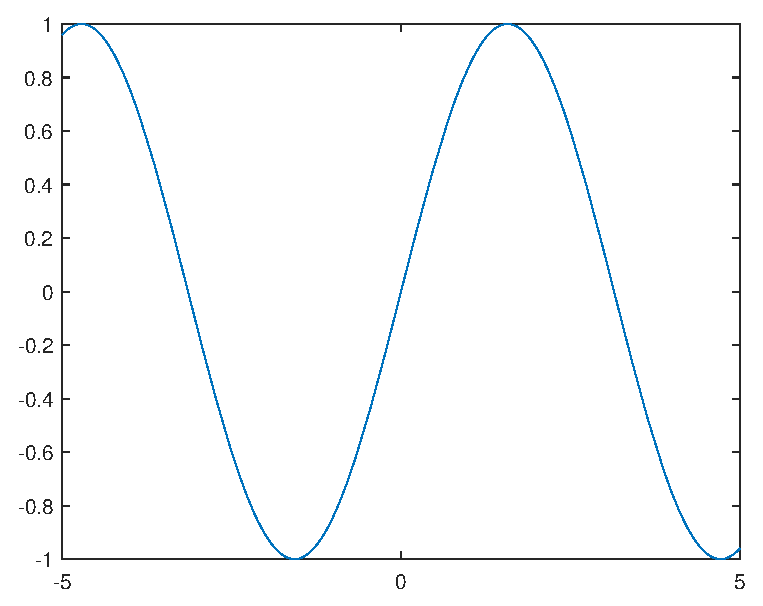
\includegraphics[width=0.45\linewidth]{image1}
  \caption{函数 $y=\sin(x)$ 的图像}\label{fig:sinx2}
\end{figure}


如下表格: 表~\ref{tab:heightweight2}. 通过 \verb|autoref| 引用表格: \autoref{tab:heightweight2}.

\begin{table}[!htp]
\centering
% PLCR已经定义
\caption{某校学生身高体重样本}
\label{tab:heightweight2}
\begin{tabularx}{0.9\textwidth}{lCCC}
   \toprule
	序号 & 年龄 & 身高 & 体重 \\
	\midrule
	001 & 15 & 156 & 42 \\
	002 & 16 & 158 & 45 \\
	003 & 14 & 162 & 48 \\
	004 & 15 & 163 & 50 \\
    \cmidrule{2-4}
	平均 & 15 & 159.75 & 46.25 \\
	\bottomrule
\end{tabularx}
\end{table}


\chapter{这是第二个附录}

\section{附录B的小节}

这里是附录环境.




%====================================%

\backmatter % 结束章节自动编号

% 攻读学位期间的研究成果
%
% 攻读学位期间的研究成果

\begin{publications}

\begin{biblist}
%\setlength{\itemsep}{3pt}
\item \textbf{Author 1} and Author 2, The name of the published article 1, \textbf{Name of Journal}, 2020, 12(34):1001--1020.

\item {\textbf{Author 1},  Author 2 and Author 3}, The name of the published article 2, submitted to Journal of XXX.
\end{biblist}

%\setlength{\hangindent}{1.6em}
%\noindent
%[1]~~{\textbf{Author 1} and Author 2}, The name of the published article 1, \textbf{Name of Journal}, 2020, 12(34):1001--1020.
%
%\setlength{\hangindent}{1.6em}
%\noindent
%[2]~~{\textbf{Author 1},  Author 2 and Author 3}, The name of the published article 2, submitted to Journal of XXX.

\end{publications}



% 致谢

%%%%%%%%%%%%%%%%%%% 致谢 %%%%%%%%%%%%%%%%%%%%%

\begin{acknowledgement}
%\setlength{\baselineskip}{24pt}
行文至此, 竟迟迟难以落笔, 思绪万千......

在晚冬的寒意还未褪去的三月初, 上海经过连续几天的下雨后终于迎来了晴天, 上天好像安排了一场见面会一样, 我毫无征兆地走进了一教215, 后知后觉想起这是我备考研究生的自习室, 在这一瞬间, 我突然觉得人生某一阶段的结束并不是消散, 而在命运的齿轮里, 研究生阶段的充实、成长和精彩已经为我的人生留下了浓墨重彩的一笔. 现回首研究生学习生涯, 皆是幸运与感恩!

得遇良师, 人之幸事. 记得第一次加上刘老师的联系方式是在本科阶段, 由于班级工作需要班导师的签名, 刘老师的礼貌和耐心给我留下了谦谦君子的印象. 进入研究生, 我非常有幸成为了刘老师的学生, 同时也成为了大家羡慕的对象, 一位性格温暖、亦师亦友、指导有方的导师成为了我研究生的指明灯. 万千言语,终将汇为一句由衷的感谢!尊敬的刘老师, 感谢您对我学术上孜孜不倦的指导和包容; 感谢您鼓励我勇敢参加学术报告提升自己; 感谢您在我在面临毕业选择时的理解和支持; 感谢您的认真负责和悉心教导让我顺利完成研究生学业......桃李不言, 下自成蹊, 感谢研究生阶段遇到的每一位老师, 愿恩师们万事胜意, 桃李芬芳.

学贵得师, 亦贵得友. 很幸运在读研期间结交了很多志同道合的好友, 有爱的同学、温暖的室友、永远默默付出的同门和师门们以及陪伴我整个青春的人, 我们一起分享着彼此的青春, 感谢你们让平淡如水的日子熠熠生辉, 愿今后的我们继续以另一种方式陪伴着彼此, 继续相伴而行. 春晖寸草, 山高海深. 我最爱的家人们, 感谢你们的陪伴与支持, 感谢你们让我永远相信即使失败也会有靠山. 亲爱的爸爸妈妈、爷爷奶奶, 一直以来辛苦您们啦, 感谢你们为我创建的幸福家庭, 我一直在享受你们无私的爱, 未来, 我们一起去看遍万千山水吧!亲爱的弟弟, 还是觉得这辈子最幸运的事是成为你的姐姐, 感谢你给我搭建的堡垒, 感谢你永远出现在我最脆弱的时侯, 感谢你带来的一切......

最后, 感谢一路坚持的自己, 蜗牛慢慢爬也会当终点的. 做好自己的事, 对生活真诚、简单和快乐, 人生终究是幸福烂漫的!



\end{acknowledgement}




\end{document}

